\section{(7) Хроматическое число гиперграфа. Пример применения ЛЛЛ для верхней оценки хроматического числа n-однородного гиперграфа в терминах максимальной степени вершины. Сравнение с тривиальной оценкой в случае обычного графа.}
$H = (V, E)$ - $n$-однородный гиперграф. (при $n = 2$ это обычный граф)
Пусть $k$ - максимальная степень вершины.

\Def Раскраска множества вершин $V$ гиперграфа $H = (V, E)$ называется правильной, если в этой раскраске все ребра из $E(H)$ не являются одноцветными. Хроматическим числом гиперграфа $H$ называется минимальное число цветов, требуемое для правильной раскраски вершин этого гиперграфа. 
\\
\\
$X(H)$ - хроматическое число гиперграфа \\
При $n = 2 \Rightarrow X(H) \leq k + 1$ (Тривиальная оценка для обычных графов) \\
При $n \geq 3 \Rightarrow X(H) \leq f(kn)$, где $f$ - какая-то функция.

\Th $e \cdot r^{1-n}(n(k-1)+1)  \leq 1 \Rightarrow X(H) \leq r$ (ничего лучшего для $n \geq 3$ сейчас не знают).

\Proof

Красим гиперграф в $r$ цветов

Красим каждую вершину в каждый конкретный цвет с вероятностью $\frac{1}{r}$.

Пусть $e_1, ..., e_{|E|}$ - рёбра гиперграфа

$A_1, ..., A_{|E|}$, где $A_i$ - событие: $e_i$ - одноцветное.

Если докажем, что $P(\bigcap_{i=1}^{|E|} \overline{A_i}) > 0$, получим $X(H) \leq r$, потому что докажем возможность покраски графа в $r$ цветов, не получив одноцветные рёбра. Докажем это:

$p = P(A_i) = r^{1-n}$

$d$ - число зависимостей. $d \leq n \cdot (k - 1)$ (Это суммарная степень всех вершин, помимо выбранного ребра(события))

По условию теоремы $e \cdot r^{1-n}(n(k-1)+1) \leq 1$, следовательно выполняется неравенство $e p (d + 1) \leq 1$. Можем воспользоваться ЛЛЛ и получить $P(\bigcap_{i=1}^{|E|} \overline{A_i}) > 0 \Rightarrow X(H) \leq r  \ \blacksquare$

$(e(n(k-1)+1))^{\frac{1}{n-1}} \leq 1 \Rightarrow X(H) \leq r$ 

$(e(n(k-1)+1))^{\frac{1}{n-1}} \leq 1 \Rightarrow r \geq \left\lceil (e(n(k-1)+1))^{\frac{1}{n-1}} \right\rceil$

И если взять в качестве $r$ значение $\left\lceil (e(n(k-1)+1))^{\frac{1}{n-1}} \right\rceil$, то оно будет удовлетворять условию $r \geq \left\lceil (e(n(k-1)+1))^{\frac{1}{n-1}} \right\rceil$ (переформулированное начальное условие), следовательно, применима теорема. Получим оценку $X(H) \leq \left\lceil (e(n(k-1)+1))^{\frac{1}{n-1}} \right\rceil$.

Если подставить n = 2 (то есть граф обычный), то получим $X(H) \leq \left\lceil e(2(k-1)+1) \right\rceil$

Эта оценка хуже, чем обычная: $X(H) \leq k + 1$, но сопостовимая.
\newpage{}

\section{(5) Двудольные числа Рамсея: нижние оценки простым вероятностным методом. Отличие нижних оценок для двудольных чисел Рамсея от аналогичных нижних оценок для $R(s, s)$.}
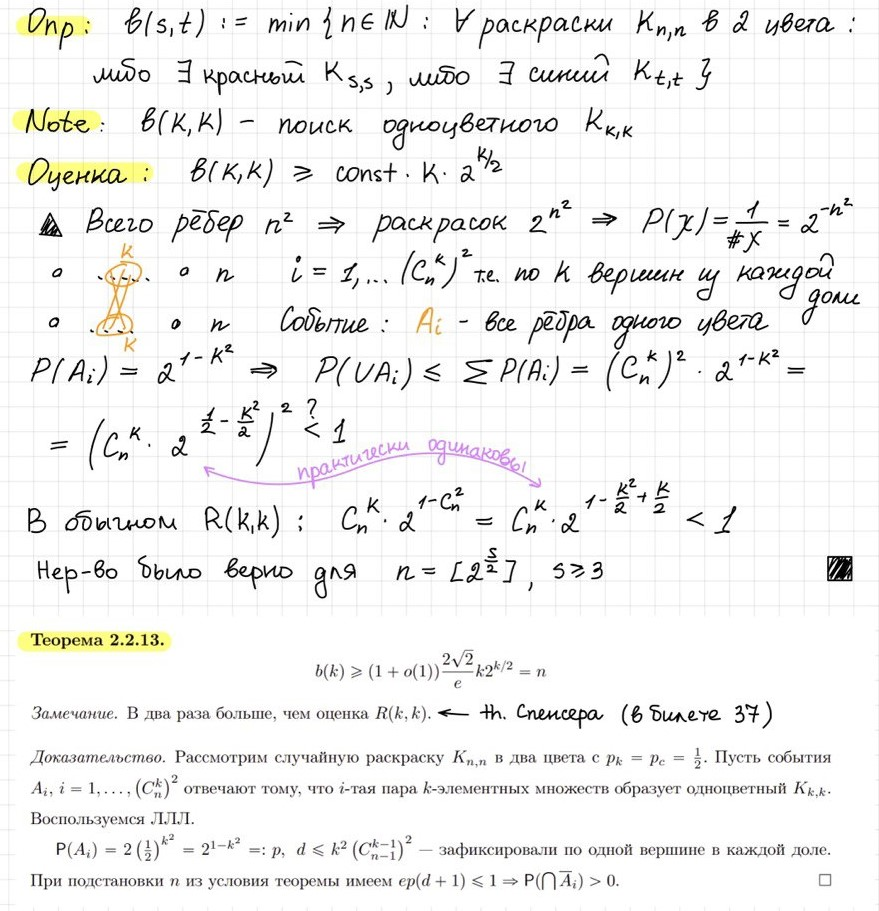
\includegraphics[width=1\linewidth]{sections/Polina/imgs/200.jpg}
\newpage{}

\section{(6) Случайные графы. Неравенства Маркова и Чебышёва. Неравенство для случайного блуждания.}
\newpage
\lecture{11}{Непрерывные цепи Маркова}
\section{Непрерывные цепи Маркова}
\subsection{Непрерывные цепи Маркова}
\begin{Def}
    Случайная функция
    \begin{align*}
      & X(t), \ t \geq 0, \ S \subseteq \ZZ, \ \left| S \right| \leq \infty
    \end{align*}
    со свойством
    \begin{align*}
      & \forall n \geq 1, \ \forall m_0 < m_1 < \dots < m_n \ \PP\left( X(t_n) = x_n \mid X(t_{n-1}) = x_{n-1}, \dots, X(t_0) = x_0 \right) = \\
      & = \PP\left( X(t_{n}) = x_n \mid X(t_{n-1}) = x_{n-1}\right)
    \end{align*}
    где эти вероятности определены, называется \textbf{непрерывной марковской
      цепью (НМЦ)}.
\end{Def}
\begin{Def}
    Если состояний конечное число, то НМЦ называется \textbf{конечной}, иначе \textbf{счетной}.
\end{Def}
\begin{Def}
    Вероятность
    \begin{align*}
      & p_{ij}(t_1,t_2) = \PP \left( X(t_1)=j \mid X(t_2) = i\right)
    \end{align*}
    назовем \textbf{вероятностью перехода из из состояния $i$ в момент $t_1$ в
      состояние $j$ в момент $t_2$} ($t_1 \leq t_2$).
\end{Def}
\begin{Def}
    Матрица
    \begin{align*}
      & P(t_1,t_2) = \left| \left| \begin{matrix} p_{ij}(t_1,t_2) \end{matrix} \right| \right|
    \end{align*}
    называется \textbf{матрицей перехода цепи от момента $t_1$ к моменту $t_2$}
    ($t_1 \leq t_2$).
\end{Def}
\textbf{Свойства}
\begin{enumerate}
    \item $\forall i \in S, \ 0 \leq s \leq t \ \dst \sum_{j \in S} p_{ij}(s,t) = 1$
    \item $\forall i \in S, \ 0 \leq t \ p_{ii}(t,t) = 1$
    \item $\forall i \neq j \in S, \ 0 \leq t \ p_{ij}(t,t) = 0$
\end{enumerate}
\begin{theorem} Уравнение Колмогорова-Чепмена
    \\
    Пусть $t_1 < t < t_2$. Тогда выполняется
    \begin{align*}
      & P(t_1,t_2) = P(t_1,t)P(t,t_2)
    \end{align*}
\end{theorem}
\begin{Proof}
    \begin{align*}
      & p_{ij}(t_1,t_2) = \PP\left( X(t_2) = j \mid X(t_1) = i \right) = \sum_{k \in S}\PP\left( X(t_2) = j \mid X(t)=k \right)\PP\left( X(t) = k \mid X(t_1) = i \right) = \\
      & = \sum_{k \in S}p_{kj}(t,t_2)p_{ik}(t,t_1)
    \end{align*}
\end{Proof}
\begin{Def}
    Вероятность $\pi_k(t) = \PP\{X_n = t\}$ называется \textbf{вероятностью
      состояния $k$ в момент $t$}.
\end{Def}
\begin{Def}
    Вектор $\pi(t) = \left[ \pi_0(t), \pi_1(t), \dots \right]^T$ называется
    \textbf{распределением вероятностей состояний в момент $t$}.
\end{Def}
\begin{theorem}
    \begin{align*}
      & \pi(t) = P(s,t)\pi(s)
    \end{align*}
\end{theorem}
\begin{Proof}
    Аналогично дискретному случаю.
\end{Proof}
\subsection{Однородные цепи Маркова}
\begin{Def}
    Если
    \begin{align*}
      & \forall t, s \geq 0 \ P(0,t) = P(s, t+s)
    \end{align*}
    то цепь Маркова называется \textbf{однородной}, иначе \textbf{неоднородной}.
\end{Def}
\begin{Des}
    Введем обозначение
    \begin{align*}
      & p_{ij}(t) = \PP\{X(t) = j\mid X(0) = i\}
    \end{align*}
\end{Des}
\begin{Def}
    Случайный процесс $\{X(t), \ t \geq 0\}$, определенный на вероятностном
    пространстве $\{\Omega, \cF, \PP\}$, называется \textbf{непрерывным справа},
    если его $\PP$-почти все траектории непрерывны справа.
\end{Def}
\begin{theorem}~
    \\
    Пусть $\{X(t), \ t \geq 0\}$~--- непрерывная справа цепь Маркова, тогда
    \begin{align*}
      & \forall s \geq 0 \ P(s,t) \To{t \to s+0} I
    \end{align*}
    В частности, для однородного процесса
    \begin{align*}
      & P(t) \To{t \to 0+0} I
    \end{align*}
\end{theorem}
\begin{Proof}
    Пусть $\{t_n\} \to s$ справа. $\forall \omega \in \Omega$ $f: t \mapsto
    X(\omega, t)$ непрерывно в $s$ справа тогда и только тогда, когда $\exists
    n_0: \forall n \geq n_0 \ X(t_n) = i$.
    \\
    Пусть $E = \{\omega\}$, для которых $f: t \mapsto X(\omega, t)$
    непрерывно в $s$ справа, тогда
    \begin{align*}
      & \left\{ \omega \in E: X(\omega,s)=i \right\} = \bigcup_{n=1}^\infty \bigcap_{k \leq n}\left\{ \omega \in \Omega: X(\omega, t_k) = i \right\}
    \end{align*}
    В силу непрерывности
    \begin{align*}
      & \mu \left( \left\{ \omega \in \Omega: X(\omega,s)=i \right\} \triangle \bigcup_{n=1}^\infty \bigcap_{k \leq n}\left\{ \omega \in \Omega: X(\omega, t_k) = i \right\} \right) = 0
    \end{align*}
    Пусть теперь
    \begin{align*}
      & \PP\{X(s) = i\} > 0
    \end{align*}
    Тогда
    \begin{align*}
      & 1 = p_{ii}(s,s) = \PP\left( X(s) = i \mid X(s) = i \right) = \PP\left( \bigcup_{n=1}^\infty \bigcap_{k \leq n}\left\{ \omega \in \Omega: X(\omega, t_k) = i \mid X(\omega, s)\right\} \right) = \lim_{n\to \infty}\PP\left( \bigcap_{k \leq n}\left\{ \omega \in \Omega: X(\omega, t_k) = i \mid X(\omega, s)\right\} \right) \leq \PP\left( X(t_n) = i \mid X(s) = i \right) \leq 1
    \end{align*}
    \begin{align*}
      & \lim_{n \to \infty} \PP\left( X(t_n) = i \mid X(s) = i \right) \leq 1
    \end{align*}
    \begin{align*}
      & p_{ii}(s,t_n) \To{n \to \infty} p_{ii}(s,s) \Rightarrow p_{ii}(s,t) \To{t \to s+0} p_{ii}(s,s)
    \end{align*}
    Далее,
    \begin{align*}
      & p_{ij}(s,t) = \PP\left( X(t) = j \mid X(s) = i \right)\leq \PP\left( X(t)\neq i \mid X(s) = i \right) = 1 - p_{ii}(s,t)
    \end{align*}
    \begin{align*}
      & p_{ij}(s,t) \To{t \to s+0} 0
    \end{align*}
    Для однородного случая
    \begin{align*}
      & P(0) = I, \ P(t+s) = P(t)P(s), \ P(t) \To{t \to 0} I
    \end{align*}
\end{Proof}
\begin{theorem}~
    \\
    Пусть $\{X(t), \ t\geq 0\}$~--- однородная НМЦ, непрерывная справа и с
    конечным числом состояний. Тогда существует матрица
    \begin{align*}
      & Q = \lim_{h \to 0+0}\frac{P(t+h)-P(t)}{h}
    \end{align*}
    а $P(t)$ удовлетворяет системе дифференциальных уравнений
    \begin{align*}
      & \dot{P(t)} = P(t)Q, \ P(0) = I \\
      & \dot{P(t)} = QP(t), \ P(0) = I
    \end{align*}
    которая имеет единственное решение
    \begin{align*}
      & P(t) = \exp\left( Qt \right)
    \end{align*}
\end{theorem}
\begin{Proof}
    В силу непрерывности $P(t)$ в нуле имеем:
    \begin{align*}
      & P(h) \To{h\to 0} I
    \end{align*}
    а значит, есть окрестность нуля такая, что $P(h)$ обратима для всех $h$ из
    неё, и
    \begin{align*}
      & P^{-1}(h) \To{h\to 0} I
    \end{align*}
    Тогда
    \begin{align*}
      & P(t+h)  = P(t)P(h) \To{t\to 0} P(t)
    \end{align*}
    \begin{align*}
      & P(t-h)  = P(t)P^{-1}(h) \To{t\to 0} P(t)
    \end{align*}
    А значит, $P(t)$ непрерывна в каждой $t$.
    \\
    Из уравнения Колмогорова-Чепмена следует
    \begin{align*}
      & P(t) = P(t-h)P(h) \Rightarrow P^{-1}(h) = P(-h)
    \end{align*}
    Более того, $P(t)$ дифференцируема для всех $t \geq 0$.
    \\
    Пусть
    \begin{align*}
      & Q = \lim_{h \to +0}\frac{P(h)-I}{h}
    \end{align*}
    Заметим:
    \begin{align*}
      & P(t+h) = P(t)P(h) = P(h)P(t) \Rightarrow \frac{P(t+h)-P(t)}{h} = P(t)\frac{P(h)+I}{h} = \frac{P(h)+I}{h}P(t)
    \end{align*}
    \begin{align*}
      & \dot{P}(t) = P(t)Q=QP(t), \ P(0) = I
    \end{align*}
    \begin{align*}
      & P(t) = \exp(Qt)
    \end{align*}
\end{Proof}
\begin{Prop}
    \begin{align*}
      & \dot{\pi}(t) = Q^T\pi(t)
    \end{align*}
\end{Prop}
\begin{Proof}
    Продифференцируем
    \begin{align*}
      & \pi(t) = P^T\pi(t)
    \end{align*}  
\end{Proof}
\begin{Def}
    Матрица $Q$ называется \textbf{матрицей интенсивностей (инфинитезимальной матрицей)}.
\end{Def}
\begin{Def}
    $q_{ij}$ называется \textbf{интенсивностью перехода из $i$ в $j$}.
\end{Def}
\begin{Prop}
    \begin{align*}
      & q_{ii} = \lim_{h \to 0+0}\frac{p_{ii}-1}{h}
    \end{align*}
    \begin{align*}
      & q_{ij} = \lim_{h \to 0+0}\frac{p_{ij}}{h}
    \end{align*}
    \begin{align*}
      & p_{ii}(h) = 1 + q_{ii}h + o(h)
    \end{align*}
    \begin{align*}
      & p_{ij}(h) = q_{ij}h + o(h)
    \end{align*}
\end{Prop}
\begin{Proof}
    \begin{align*}
      & \sum_{j}p_{ij}(h) = 1
    \end{align*}
    \begin{align*}
      & 1 = 1+q_{ii}h+o(h)+\sum_{i\neq j}q_{ij}h+o(h)
    \end{align*}
    \begin{align*}
      & \sum_{i\neq j}q_{ij} = -q_{ii}
    \end{align*}    
\end{Proof}
\begin{Def}
Пусть $\{X(t), t \geq 0\}$~--- однородная НМЦ с конечным или счетным числом
состояний, непрерывными справа траекториями. Определим \textbf{время пребывания
  в состоянии $i \in S$} по формуле
\begin{align*}
  & \tau_i(\omega) = \inf\left( t: X(\omega, t) \neq i \right)
\end{align*}
\end{Def}
\begin{Prop}
    Для таких процессов
    \begin{align*}
      & \tau_i(\omega) = \inf\left( t: X(\omega, t) \neq i \right) = \inf\left( t \in D: X(\omega, t) \neq i \right) = \tau_i^D, \ \left| D \right| = \aleph_0, \ [D] = \RR
    \end{align*}
    почти наверное.
\end{Prop}
\begin{Proof}
    Очевидно,
    \begin{align*}
      & \tau_i \leq \tau_i^D
    \end{align*}
    Если $\tau_i = +\infty$, то $\tau_i^D = +\infty$. Иначе в силу всюду
    плотности есть последовательность $\{t_n\} \to \tau_i$. Но тогда в силу
    непрерывности справа $X(\omega, \tau_i(\omega)) \neq i$, а значит,
    \begin{align*}
      & \tau_i \geq \tau_i^D
    \end{align*}  
\end{Proof}
Будем рассматривать $\tau_i^D(\omega)$, являющийся случайной величиной.
\\
В качестве $D$ удобно брать
\begin{align*}
  & D_t = \bigcup_{n=0}^\infty D_n = \bigcup_{n=0}^\infty \left\{ \frac{jt}{2^n} \right\}^{2^n}_{j=0}; \ D_n \subseteq D_{n+1}
\end{align*}
\begin{align*}
  & \PP\left( \tau_i^D>t \right)  = \PP\left( \bigcap_{n=0}^\infty \bigcap_{j=0}^{2^n} \left\{ X\left( \frac{jt}{2^n} \right) = i \right\} \right) = \lim_{n \to \infty}\left( \bigcap_{j=0}^{2^n} \left\{ X\left( \frac{jt}{2^n} \right) = i \right\} \right) = \lim_{n \to \infty} p_{ii}^{2n}\left( \frac{t}{2^n} \right) \cdot \\
  & \cdot \pi_i(0) = \lim_{n \to \infty} \left( 1+p_{ii}\left( \frac{t}{2^n} \right) +o\left( \frac{t}{2^n} \right)\right)^{2^n}\pi_i(0) = e^{q_{ii}t}\pi_i(0)
\end{align*}
\begin{Note}
    Если цепь стартует из $i$, то время пребывания в состоянии $i$ имеет
    экспоненциальное распределение интенсивности $-q_{ii}$
\end{Note}
\begin{Des}
    Пуусть
    \begin{align*}
      & q_i = -q_{ii} = \sum_{j \neq i}q_{ij}
    \end{align*}
\end{Des}
\begin{Note}
    \begin{align*}
      & \pi_i(0) = 1 \Rightarrow \tau_i^D \in Exp(q_i)
    \end{align*}
\end{Note}
\begin{Des}
    Пусть
    \begin{align*}
      & F_{ij}(h) = \PP\left( X(t+h) = j\mid X(t) = i, X(t+h) \neq i \right)
    \end{align*}
\end{Des}
Тогда по определению условной вероятности
\begin{align*}
  & f_{ij}(t+h) = \frac{\PP\left( X(t+h) = j\mid X(t) = i \right)}{\PP\left( X(t+h) \neq i \mid X(t) = i \right)}\To{h \to 0} \frac{q_{ij}}{q_i}
\end{align*}
\begin{Def}
    $\dst \frac{q_{ij}}{q_i}$~--- вероятность перейти из $i$ в $j$ в момент прыжка.
\end{Def}
Пусть цепь стартует из $i$ и находится там $Exp(q_i)$ времени, и цепь попадает в
$j$ с вероятностью $\dst \frac{q_{ij}}{q_i}$, потом спустя $Exp(q_j)$ происходит
ещё один прыжок и так далее.
\newpage{}

\section{(7) Связность случайного графа: случай $p = c \frac{\ln n}{n}$ при $c < 1$. Теоремы о $\frac{\ln n + \gamma}{n}$ и о гигантской компоненте (б/д).}
\Th Пусть $G(n, p)$ $-$ случайный граф, $p = c \frac{\ln n}{n}$. \\
$1.$ Если $c > 1$, то а. п. н. G связен; \\
$2.$ Если $c < 1$, то а. п. н. G несвязен.

\underline{Доказательство пункта 2}: \\
\Proof Пусть $X=X(G)$ $-$ количество изолированных вершин в графе G. Тогда
$$\mathbb{P}(X \geqslant 1)=1 - \mathbb{P}(X \leqslant 0) = 1 - \mathbb{P}(-X \geqslant 0)=1-\mathbb{P}(\mathbb{E}X - X \geqslant \mathbb{E}X) \geqslant 1 - \mathbb{P}(|\mathbb{E} X - X| \geqslant \mathbb{E} X) \geqslant 1 - \frac{\mathbb{D} X}{(\mathbb{E}X)^2}$$

Из линйености мат. ожидания $\mathbb{E} X = \mathbb{E} \sum^n_{i=1} X_i=n(1-p)^{n-1}$, где $X_i$ - изолирована ли i-я вершина. Далее найдём $\mathbb{E}X^2$:
$$\mathbb{E}X^2 = \mathbb{E} \left( \sum^n_{i=1} X_i \right)^2 = \mathbb{E}X + \sum_{i \neq j}\mathbb{E}(X_i X_j) = \mathbb{E}X + n(n-1)(1-p)^{2n-3}$$

Подставив вероятность, получим
$$\mathbb{E} X = n(1-p)^{n-1} = n e^{(n-1)\ln(1-p)} = n e^{-(1 + \overline{\overline{o}}(1))n p} = n e^{-(1 + \overline{\overline{o}}(1))c \ln n} = n \frac{1}{n^{c(1 + \overline{\overline{o}}(1))}} \xrightarrow[n \rightarrow{\infty}] {}\infty$$

Тогда можно записать следующее:
$$\frac{\mathbb{D} X}{(\mathbb{E}X)^2} = \frac{\mathbb{E}X}{(\mathbb{E} X)^2} + \frac{n(n-1)(1-p)^{2n-3}}{(\mathbb{E} X)^2} - \frac{(\mathbb{E} X)^2}{(\mathbb{E} X)^2} \xrightarrow[n \rightarrow{\infty}]{} 0 + \left( \frac{n(n-1)(1-p)^{2n-3}}{n^2(1-p)^{2n-2}} \sim \frac{1}{1-p} \sim 1 \right) - 1 = 0$$

Тогда, подставив это в первую формулу, получим, что а. п. н. в графе будет хотя бы одна изолированная вершина, значит, он будет несвязным. \EndProof


\underline{Дополнительные оценки}: \\
$1.$ Если $c=1$, то вероятность G быть связным равна $\frac{1}{e}$; \\
$2.$ Если $p=\frac{\ln n + \gamma}{n}$, то вероятность G быть связным стремится к $e^{-e^{-\gamma}}$. 

\textbf{Теорема(о гигантской компоненте):} Пусть $p=\frac{c}{n}$, $c > 0$. \\
$1.$ Если $c < 1$, то $\exists \beta > 0$, такая что а. п. н. размер каждой компоненты связности  не превосходит $\beta \ln n$; \\
$2.$ Если $c > 1$, то $\exists \beta > 0 \wedge \exists \gamma \in (0; 1)$, такие что а. п. н. ровно одна компонента связности имеет $\geqslant \gamma n$ вершин, а размер всех остальных не превосходит $\beta \ln n$.
\newpage{}

\section{(8) Связность случайного графа: случай $p = c \frac{\ln n}{n}$ при $c > 1$.}
\Th Пусть $G(n, p)$ $-$ случайный граф, $p = c \frac{\ln n}{n}$. \\
$1.$ Если $c > 1$, то а. п. н. G связен; \\
$2.$ Если $c < 1$, то а. п. н. G несвязен.

\underline{Доказетальство пункта 1}:

\Proof $\mathbb{P}(G(n, p)\: \text{не связен}) = \mathbb{P}(\exists k \in \overline{1..(n-1)}\! \wedge\! \exists W \subset \overline{1..n}: |W|=k\! \wedge\! G \big|_W\: \text{связен и}\: \forall x \notin W\: \text{нет рёбер из } x\: \text{в}\: W) \leqslant \sum^{n-1}_{k=1} \sum_{W:|W|=k} \mathbb{P}(\forall x \notin W \forall y \in W (\{ x, y\} \notin E)) = \sum^{n-1}_{k=1}C^k_n(1-p)^{k(n-k)}$. Назовём выражение под суммой $a_k(n)$. Нам известно, что $a_1(n) \rightarrow 0$. Заметим, что слагаемые симметричны относительно n/2, поэтому достаточно будет оценить только первую половину суммы. Разобьём её на две части: $\sum^{n/2}_{k=1}... = \sum^{n/\sqrt{\ln n}}_{k=1}... + \sum^{n / 2}_{k=n/\sqrt{\ln n} + 1}...$

Заметим, что $C^k_n(1-p)^{k(n-k)} < 2^n e^{-pk(n-k)} \leqslant 2^n e^{-pk\frac{n}{2}} < 2^n e ^{-p \frac{n^2}{2 \sqrt{\ln n}}} = e^{n \ln 2 - c\sqrt{\ln n} \frac{n}{2}} \xrightarrow[n \rightarrow \infty]{} 0$. Значит, вторая сумма стремится к 0.

Теперь заметим, что $\frac{a_{k+1}(n)}{a_k(n)} = \frac{C^{k+1}_n(1-p)^{(k+1)(n-k-1)}} {C^{k}_n(1-p)^{(k)(n-k)}} = \frac{n-k}{k+1}(1-p)^{n-2k-1} \sim \frac{n-k}{k+1}(1-p)^{n-2k} < n(1-p)^{n-2k} < n(1-p)^{n - n / \sqrt{\ln n}}=q(n)$.

Значит, первая сумма расписывается как $\sum^{n / \sqrt{\ln n}}_{k=1} C^k_n (1-p)^{k(n-k)} \cdot (1 + q(n) + q^2(n) + ...) < n(1-p)^{n-1} \cdot \frac{1}{1-q(n)} \xrightarrow[n \rightarrow\infty]{} 0$

Таким образом, обе части суммы стремятся к 0, значит и вся сумма стремится к 0 с ростом n. \EndProof

\newpage{}

\section{(5) Теоремы Боллобаша о хроматическом числе случайного графа (б/д). Оценки хроматического числа случайного графа при $p = o(\frac{1}{n^2})$ и $p = o(\frac{1}{n})$.}
\newpage
\lecture{12}{Непрерывные цепи Маркова (продолжение)}
\begin{Def}
    \textbf{Прямое уравнение Колмогорова}
    \begin{align*}
      & \dot{P}(t) = P(t)Q
    \end{align*}
\end{Def}
\begin{Def}
    \textbf{Обратное уравнение Колмогорова}
    \begin{align*}
      & \dot{P}(t) = QP(t)
    \end{align*}
\end{Def}
\subsection{Эргодические непрерывные цепи Маркова}
\begin{Def}
    Распределение $\pi^0$ называется \textbf{стационарным}, если
    \begin{align*}
      & \forall t \geq 0 \ P^T(t)\pi^0 = \pi^0
    \end{align*}
\end{Def}
\begin{Def}
    Для стационарного
    \begin{align*}
      & \dot{\pi}(t) = Q^T\pi(t) \Rightarrow 0 = Q^T\pi^0(t)
    \end{align*}
    \textbf{стационарные уравнения Колмогорова.}
\end{Def}
\begin{Def}
    Если
    \begin{align*}
      & \exists t > 0: \ p_{ij}(t) > 0
    \end{align*}
    то говорят, что \textbf{за $i$ следует $j$}.
\end{Def}
\begin{Def}
    Если $i \rightarrow j$ и $j \rightarrow i$, то говорят, что \textbf{$i$ и
      $j$~--- сообщающиеся}.
\end{Def}
Отношение делит цепь на \textbf{классы сообщающихся состояний}.
\begin{Def}
    Если
    \begin{align*}
      \forall j \in S \ (i \rightarrow j) \rightarrow (j \rightarrow i)
    \end{align*}
    то говорят, что \textbf{$i$~--- существенное состояние}, иначе
    \textbf{несущественное}.
\end{Def}
\begin{Def}
    Если $\dst \lim_{t \to \infty} p_{ii}(t) = 0$, то состояние $i$ называется
    \textbf{нулевым}, иначе \textbf{ненулевым}.
\end{Def}
\begin{Def}
    Если все состояния сообщаются, то цепь называется \textbf{неразложимой
      (неприводимой)}.
\end{Def}
\begin{Des}
    Обозначим вероятность возврата в $i$ за конечное время
    \begin{align*}
      & F_i = \int_0^{\infty}f_i (t)dt
    \end{align*}
\end{Des}
\begin{Def}
    Если $F_i = 1$, то состояние $i$ наывается \textbf{возвратным}, иначе
    \textbf{невозвратным}.
\end{Def}
\begin{theorem} (о солидарности)
    \\
    Для неразложимых марковских цепей выполняется:
    \begin{enumerate}
        \item Если есть хотя бы одно нулевое состояние, то нулевыми будут все;
        \item Если есть хотя бы одно возвратное состояние, то возвратными будут
        все.
    \end{enumerate}
\end{theorem}
\begin{Def}
    ДМЦ, у которой
    \begin{align*}
      & p_{ij} = \begin{cases}
          \dst \frac{q_{ij}}{q_i}, \ i \neq j \\
          0, \ i = j
          \end{cases}
    \end{align*}
    называется \textbf{цепью скачков}.
\end{Def}
\begin{Def}
    Марковская цепь называется \textbf{эргодической}, если $\forall i,j \in S \
    \exists \dst \lim_{t\to \infty}p_{ij}(t) = p_j > 0$, не зависящий от $i$.
\end{Def}
\begin{theorem} Эргодическая для конечных цепей
    \\
    Для эргодичности конечной непрерывной цепи Маркова необходимо и достаточно
    наличие неразложимости.
\end{theorem}
\begin{Proof}
    Докажем <<идейно>>.
    \begin{itemize}
        \item Непрерывность.
        \\
        Аналогично дискретной.
        \item Достаточность.
        \\
        Заметим, что в силу неразложимости $\forall t \geq 0 \ p_{ij}(t)>0$.
        \\
        В силу экспоненциального распределения и сообщаемости вероятность
        попасть в любое состояние из любого за сколь угодно малое время не ноль;
        далее доказываем точь-в-точь как для дискретной цепи.
    \end{itemize}
\end{Proof}
\begin{theorem} (о предельном распределении)
    \\
    В конечных эргодических цепях
    \begin{enumerate}
        \item $\exists C > 0, \ \rho \in (0;1): \ \forall t \geq 0 \ \left| p_{ij}(t) \right| \leq
        C\rho^t$;
        \item числа $p_{j}$ задают распределение состояний;
        \item это распределение стационарно;
        \item это стационарное распределение~--- единственное стационарное
        распределение для данной цепи Маркова;
        \item $\forall j \ \pi_{j}(t) \To{n \to \infty} p_j$
    \end{enumerate}
\end{theorem}
\begin{Proof}
    Доказательство проводим точь-в-точь как для непрерывного случая.
\end{Proof}
\begin{theorem} (без доказательства)
    \\
    В конечной непрерывной эргодической цепи Маркова
    \begin{align*}
      & \frac{1}{T}\int_{0}^T\chi_{X(t)=i}dt \os{\text{п.~н.}}{\To{t\to \infty}}p_j
    \end{align*}
\end{theorem}
\subsection{Процессы гибели и рождения}
\begin{Def}
    Однородная непрерывная марковская цепь называется \textbf{процессом гибели и
      рождения}, если ее стохастический граф имеет вид
    (число состояний может быть конечным или бесконечным).
\end{Def}
\begin{Def}
    $\lambda_j$~--- \textbf{интенсивности рождения}.
\end{Def}
\begin{Def}
    $\mu_j$~--- \textbf{интенсивности гибели}.
\end{Def}
\begin{theorem} (без доказательства)
    \\
    Пусть $X(t)$~--- конечный процесс гибели и рождения, $\lambda_j, \mu_j > 0$.
    Тогда стационарное распределение существует, единственно и определяется
    соотношениями
    \begin{align*}
      & \pi_0^0 = \left( \sum_{i=0}^N \prod_{j=0}^i \frac{\lambda_j}{\mu_j} \right)^{-1} \\
      & \pi_j^0 = \frac{\lambda_j}{\mu_j}\pi_{j-1}^0
    \end{align*}
\end{theorem}
\begin{Def}
    Если все $\lambda_j = 0$, то это \textbf{процесс (чистой) гибели}.
\end{Def}
\begin{Def}
    Если все $\mu_j = 0$, то это \textbf{процесс (чистого) рождения}.
\end{Def}
\subsection{Взрывные марковские цепи}
\begin{Des}
    Пусть $T_n, \ n \geq 1$~--- моменты времени, когда осуществляются переходы
    между состояниями, $T_{\infty} = \dst \lim_{n \to \infty} T_n$.
\end{Des}
\begin{Des}
    Если
    \begin{align*}
      & \forall i \in S \ \PP\left( T_\infty = \infty \mid X(0) = i \right) = 1
    \end{align*}
    то это \textbf{невзрывная}, иначе \textbf{взрывная} марковская цепь.
\end{Des}
Бесконечное число переходов за конечное время.
\begin{theorem}
    Пусть $\{\xi_n\} \in Exp(\lambda_n)$ независимы. Тогда
    \begin{align*}
      & \sum_{j=1}^N\frac{1}{\lambda_j} = \infty \Rightarrow \PP\left( \sum_{j=1}^N \xi_j =\infty \right) =1
    \end{align*}
    \begin{align*}
      & \sum_{j=1}^N\frac{1}{\lambda_j} < \infty \Rightarrow \PP\left( \sum_{j=1}^N \xi_j <\infty \right) =1
    \end{align*}
\end{theorem}
\begin{Proof}
    Пусть
    \begin{align*}
      & \sum_{j=1}^N\frac{1}{\lambda_j} = \EE \sum_{j=1}^N \xi_j < \infty \Rightarrow \PP\left( \sum_{j=1}^N \xi_j <\infty \right) =1
    \end{align*}
    Пусть
    \begin{align*}
      & \sum_{j=1}^\infty\frac{1}{\lambda_j} = \infty
    \end{align*}
    Тогда
    \begin{align*}
      & \EE \exp\left( -\sum_{j=1}^\infty\xi_j\right) = \prod_{j=1}^\infty \EE \exp \left( -\xi_j \right) = \prod_{j=1}^\infty \left( 1 + \frac{1}{\lambda_n} \right)^{-1} = 0
    \end{align*}
    \begin{align*}
      & \PP\left( \sum_{j=1}^N \xi_j =\infty \right) = 1
    \end{align*}
\end{Proof}
\begin{corollary}
    Процесс рождения с интенсивностями $\lambda_j$ является взрывным тогда и
    только тогда, когда
    \begin{align*}
      & \sum_{j=1}^N\frac{1}{\lambda_j} < \infty
    \end{align*}
\end{corollary}
\begin{Note}
    Пуассоновский процесс есть непрерывный невзрывной процесс рождения.
\end{Note}
\subsection{Потоки событий}
\begin{Def}
    \textbf{Поток событий}~--- последовательность одинаковых событий,
    происходящих одно за другим через промежутки времени случайной длины.
\end{Def}
\begin{Des}
    Пусть $n(t_1,t_2)$~--- число событий из потока, произошедщших на промежутке
    $[t_1, t_2)$.
\end{Des}
\begin{Def}
    Предположим, что для всех $t$ существует и конечен предел
    \begin{align*}
      & \lambda(t) = \lim_{n \to 0}\frac{P(n(t,t+h) > 0)}{h}
    \end{align*}
    Он называется \textbf{интенсивностью потока событий.}
\end{Def}
\begin{Def}
    Потко называется \textbf{однородным (стационарным)}, если законы
    распределения $n(t_1,t_2)$ и $n(t_1+s, t_2+s)$ совпадают для всех $s \geq
    0$.
\end{Def}
\begin{Des}
    Для однородных потоков
    \begin{align*}
      & \PP\left( n(s,s+t) = m \right) = \PP\left( n(0,t) = m \right)
    \end{align*}
    и обозначим
    \begin{align*}
      & \eta(t) = n(0, t)
    \end{align*}
    а
    \begin{align*}
      & \lambda(t) = \lim_{n \to 0}\frac{P(n(t,t+h) > 0)}{h} = \lim_{n \to 0}\frac{P(n(0,h) > 0)}{h} = \lambda(0) = \lambda
    \end{align*}  
\end{Des}
\begin{Def}
    Поток называется \textbf{ординарным}, если
    \begin{align*}
      & \forall t \geq 0, \ h > 0 \ \PP\left( n(t,t+h) = 1 \right) = \lambda(t)h+o(h), \ h \to 0
    \end{align*}
    \begin{align*}
      & \forall t \geq 0, \ h > 0 \ \PP\left( n(t,t+h) > 1 \right) = o(h), \ h \to 0
    \end{align*}
\end{Def}
\begin{corollary}
    \begin{align*}
      & \forall t \geq 0, \ h > 0 \ \PP\left( n(t,t+h) = 0 \right) = 1-\lambda(t) h + o(h), \ h \to 0
    \end{align*}
\end{corollary}
\begin{Prop}
    Для ожнородного потока
    \begin{align*}
      & \forall t \geq 0, \ h > 0 \ \PP\left( n(t,t+h) = 1 \right) = \lambda h+o(h), \ h \to 0
    \end{align*}
    \begin{align*}
      & \forall t \geq 0, \ h > 0 \ \PP\left( n(t,t+h) = 0 \right) = 1 - \lambda h+o(h), \ h \to 0
    \end{align*}
\end{Prop}
\begin{Def}
    Рассмотрим $0 \leq t_1 \leq \dots \leq t_{m+1}$, $\xi_k = n(t_k,t_{k+1})$.
    Если эти величины независимы в совокупности, то поток называется
    \textbf{потоком без последействия.}
\end{Def}
\begin{Prop}
    Рассмотрим ординарный поток без последействия $X(t) = n(0,t)$. У него
    независимы приращения, а значит, он марковский. Его множество состояний есть
    $\NN_0$, а значит, это марковская цепь. Пусть между событиями обязательно
    происходит конечное время. Если процесс однороден, то и цепь однородна с
    интенсивностями перехода между состояниями $\lambda$.
    \\
    Это будет являться пуассоновским процессом.
\end{Prop}
\begin{Def}
    Ординарный поток без последействия называют \textbf{пуассоновским потоком
      событий}.
\end{Def}
\begin{Def}
    Однородный пуассоновский поток называют \textbf{простейшим потоком событий}.
\end{Def}
\subsection{Эквивалентные определения пуассоновского процесса}
\begin{enumerate}
    \item Первый подход.
    \begin{Def}
        Случайная функция $\left\{ K(t) \mid t \geq 0 \right\}$ называется
        \textbf{пуассоновским процессом интенсивности $\lambda$}, если
        \begin{enumerate}
            \item $K(0) = 0$ почти наверное;
            \item $K(t)$~--- процесс с независимыми приращениями;
            \item $\forall t > s \geq 0$ $K(t) - K(s) \in Po(\lambda(t-s))$
        \end{enumerate}
    \end{Def}
    \item Второй подход.
    \begin{Def} Пусть $\{\xi_n\}$~--- последовательность независимых случайных
        величин с распределением $Exp(\lambda)$. Обозначим
        \begin{align*}
          & S_0 = 0, \ S_n = \sum_{i=1}^n \xi_i
        \end{align*}
        Введём процесс
        \begin{align*}
          & X(t) = \sup \{n \mid S_n \leq t\}
        \end{align*}
        Это будет пуассоновский с параметром $\lambda$ процесс.
    \end{Def}
    \item Третий подход.
    \begin{Def}
        Пусть $K(t), \ t \geq 0$~--- непрерывная марковская цепь с $S = \NN_0$,
        непрерывным временем, непрерывная справа, процесс чистого рождения
        интенсивности $\lambda$. Тогда это пуассоновский процесс интенсивности
        $\lambda$.
    \end{Def}
    \item Четвертый подход.
    \begin{Def}
        Пусть дан простейший пуассоновский поток событий. Тогда $K(t) = n(0,t)$
        будет пуассоновским процессом.
    \end{Def}
\end{enumerate}
\newpage{}

\section{(10) Оценка отклонения для липшицевой по вершинам случайной величины (б/д). Теорема Боллобаша о хроматическом числе при $p = n^{-\alpha}$ (б/д): техническая лемма с доказательством.}
\par \Def Пусть $\Omega$ - множество всех графов на $n$ вершинах. Случайная величина $f: \Omega \rightarrow \mathbb{R}$ называется липшицевой по ребрам (по вершинам), если $|f(G)-f(G')|\leq 1$, коль скоро $G$ и $G'$ отличаются только в одном ребре (только в окрестности одной вершины).

\par \Example $\chi$ - липшицева по вершинам (а следовательно и по ребрам). Количество треугольников - не липшицева.

\par \textbf{Неравенство Азумы (оценка уклонения):} Пусть $f$ - липшицева по вершинам. Тогда $$\forall a > 0 \hookrightarrow P(|f-\mathbb{E}f| \geq a) \leq 2e^{-\frac{a^2}{2(n-1)}}$$

\par \Note Для вероятности без модуля справедливо такое же неравенство, но без множителя 2

\par \textbf{Теорема (Боллобаш):} Пусть $p=p(n)=n^{-\alpha}$, где $\alpha \in \left(\frac{1}{2}; 1\right)$. Тогда $\exists u: u = u(n, \alpha)\rightarrow \infty$ при $n\rightarrow\infty$: а.п.н. $\chi(G) \in \{u; u+1\}$.

\par \Note Интуитивно: хроматическое число концентрируется в двух значениях. Мы будем доказывать для $\alpha > \frac{5}{6}$ и $\chi(G) \in \{u, u+1, u+2, u+3\}$.

\par \Lemma Пусть $p=n^{-\alpha}, \alpha>\frac{5}{6}$. Тогда $$\exists n_0: \forall n \geq n_0 \hookrightarrow P(\forall S \subset \{1, \ldots, n\}, |S|\leq \sqrt{n}\ln{n}: \chi(G|_S) \leq 3) \geq 1-\frac{1}{\ln{n}}$$

\par \Proof Докажем, что для отрицания этого события вероятность $\leq \frac{1}{\ln{n}}$, начиная с какого-то $n$. Отрицание: $$P(\exists S, |S| \leq \sqrt{n}\ln{n}: \chi(G|_S) \geq 4)=P(\exists S, 4 \leq |S| \leq \sqrt{n}\ln{n}: \chi(G|_S) \geq 4 \text{, но }\exists x \in S: \chi(G|_{S\setminus \{x\}}) \leq 3)$$ \par Интуитивно: существует $S \Leftrightarrow$ существует минимальное по включению $S$. Обозначим эту вероятность как $P(A)$

\par Степень любой вершины $x \in S$ в $S$ больше 2, так как иначе при ее добавлении к $S\setminus \{x\}$ хроматическое число не подимется от $\leq 3$ до $\geq 4$ (если соседа всего 2, красим $x$ в незанятый цвет). Тогда количество ребер в индуцированном подграфе: $|E(G|_S)|\geq \frac{3|S|}{2}$

\par Введем новое событие $B = \exists s \in [4; \sqrt{n} \ln{n}], \exists S: |S|=s: |E(G|_S)|\geq \frac{3|S|}{2}$. $B$ следует из $A$ (из соображений выше). Тогда $$P(A) \leq P(B) \leq \sum_{s=4}^{\sqrt{n}\ln{n}} \sum_{S \subset \{1, \ldots, n\}, |S|=s} P(|E(G|_S)|\geq \frac{3|S|}{2})=*$$

\par Событие в последней сумме: в $S$ есть хотя бы $\frac{3s}{2}$ ребер. Его вероятность легко считается

$$*=\sum_{s=4}^{\sqrt{n}\ln{n}} \sum_{S \subset \{1, \ldots, n\}, |S|=s} C_{C_s^2}^{\frac{3s}{2}} p^{\frac{3s}{2}}=\sum_{s=4}^{\sqrt{n}\ln{n}} C_n^s C_{C_s^2}^{\frac{3s}{2}} p^{\frac{3s}{2}}=*$$

\par Воспользуемся неравенством $$C_a^b \leq \frac{a^b}{b!}; \: b! \geq \left(\frac{b}{e}\right)^b \Rightarrow C_a^b \leq \left(\frac{ea}{b}\right)^b$$

$$* \leq \sum_{s=4}^{\sqrt{n}\ln{n}} \left(\frac{en}{s}\right)^s \left(\frac{eC_s^2}{3s/2}\right)^{\frac{3s}{2}} p^{\frac{3s}{2}} < \sum_{s=4}^{\sqrt{n}\ln{n}} \left(\frac{en}{s}\right)^s s^{\frac{3s}{2}} p^{\frac{3s}{2}} = *$$

\par Последний переход получили из того, что $\frac{C_s^2}{s/2} < s$ + откинули $(e/3)^{\frac{3s}{2}} < 1$. Так как $s \leq \sqrt{n}\ln{n}$ и $p=n^{-\alpha}$ получим

$$*=\sum_{s=4}^{\sqrt{n}\ln{n}} \left(\frac{en}{s}s^{\frac{3}{2}}p^{\frac{3}{2}}\right)^s \leq \sum_{s=4}^{\sqrt{n}\ln{n}} \left( en (\sqrt{n}\ln{n})^{1/2} n^{-\frac{3}{2}\alpha}\right)^s=*$$

\par Введем $\beta = -\left(\frac{5}{4}-\frac{3}{2}\alpha\right) > 0$ при $\alpha > \frac{5}{6}$. Тогда

$$*=\sum_{s=4}^{\sqrt{n}\ln{n}} (en^{-\beta}\sqrt{\ln{s}})^s \underset{n \geq n_1}{<} \sum_{s=4}^{\sqrt{n}\ln{n}} (n^{-\frac{\beta}{2}})^s \leq n^{-2\beta} \left(\frac{1}{1-n^{-\beta/2}}\right) \underset{n \geq n_0}{<} \frac{1}{\ln{n}} \: \blacksquare$$


\newpage{}

\section{(10) Оценка отклонения для липшицевой по вершинам случайной величины (б/д). Теорема Боллобаша о хроматическом числе при $p = n^{-\alpha}$: техническая лемма (б/д), вывод теоремы из технической
леммы.}
\par Все формулировки см. в прошлом билете (46)

\par \textbf{Вывод теоремы из леммы:} \Proof Зафиксируем $a > \frac{5}{6}, n \geq n_0' \geq n_0$. Определим $u=u(n, \alpha)$ - минимальное число, такое что $P(\chi(G) \leq u) > \frac{1}{\ln{n}}$ (для $u=n$ условие точно выполнено. Будем уменьшать $u$ пока оно не нарушится). Тогдв $P(\chi(G) \leq u-1) \leq \frac{1}{\ln{n}}$ (иначе могли бы уменьшить $u$), а значит $P(\chi(G) \geq u) \geq 1-\frac{1}{\ln{n}}$.

\par Введем случайную величину $Y(G):=\min \{k: \exists S \subset \{1, \ldots, n\}, |S|=k: \chi(G|_{\{1, \ldots, n\} \setminus S}) \leq u)\}$ (размер самого маленького кусочка, который можно выкинуть, чтобы граф покрасился в $u$ цветов). Эта случайная величина липшицева по вершинам (если портим что-то в окрестности одной вершины в худшем случае меняется только покраска этой вершины, так что размер минимального кусочка который надо выкинуть изменится не больше чем на 1).

\par Возьмём $a=\sqrt{2(n-1)\ln{\ln{n}}}$. Тогда из неравенства Азумы: $$P(Y-\mathbb{E}Y \leq -a)=P(Y-\mathbb{E}Y \geq a)\leq e^{-\frac{a^2}{2(n-1)}}=\frac{1}{\ln{n}}$$

\par Предположим, что $\mathbb{E}Y\geq a$. Тогда $P(Y-\mathbb{E}Y \leq -a) \leq \frac{1}{\ln{n}}$ (неравенство Азумы). С другой стороны, $P(Y-\mathbb{E}Y \leq -a) = P(Y \leq \mathbb{E}Y-a)$. Так как $\mathbb{E}Y-a \geq 0$, эта вероятность $\geq P(Y \leq 0)$. Это событие равноценно тому, что для того чтобы покрасить в $u$ цветов из графа ничего не надо удалять, то есть эта веротяность $=P(\chi(G) \leq u)>\frac{1}{\ln{n}}$ (последнее неравенство из определения $u$). Получили, что вероятность одновременно и больше и меньше $\frac{1}{\ln{n}}$ - противоречие. Следовательно $\mathbb{E}Y < a$.

$$\frac{1}{\ln{n}} \geq P(Y-\mathbb{E}Y \geq a)=P(Y \geq \mathbb{E}Y + a) \geq P(Y \geq 2a)=$$ 

\par Последнее неравенство следует из того, что $\mathbb{E}Y+a < 2a$.
$$=P(Y \geq 2\sqrt{2(n-1)\ln{\ln{n}}})\underset{n \geq n_0'}{\geq} P(Y > \sqrt{n} \ln{n})$$

\par Последний переход справедлив потому что $2\sqrt{2(n-1)\ln{\ln{n}}}$ асимптотически меньше $\sqrt{n} \ln{n}$. Таким образом получаем три события

$$P(A):=P(\chi(G) \geq u) > 1-\frac{1}{\ln{n}} \text{ (из начала доказательства)}$$
$$P(B):=P(\forall S \subset \{1, \ldots, n\}, |S|\leq \sqrt{n}\ln{n}: \chi(G|_S) \leq 3) \geq 1-\frac{1}{\ln{n}} \text{ (из технической леммы)}$$
$$P(C):=P(Y \leq \sqrt{n} \ln{n}) \geq 1 - \frac{1}{\ln{n}}$$

\par Рассмотрим $G \in A \cap B \cap C$
\begin{enumerate}
    \item $\chi(G) \geq u$, так как $G \in A$
    \item $Y(G) \leq \sqrt{n} \ln{n}$, так как $G \in C$ (то есть можно выделить такое множество $S, |S| \leq \sqrt{n}\ln{n}$, что все кроме него красится в $u$ цветов). 
    \item $G \in B \Rightarrow S$ можно покрасить в 3 цвета $\Rightarrow \chi(G) \leq u+3$    
\end{enumerate}

\par Значит $u \leq \chi(G) \leq u+3$. Так как $P(A \cap B \cap C) = 1 - P(\overline{A} \cup \overline{B} \cup \overline{C}) \geq 1 - \frac{3}{\ln{n}}\rightarrow 1$, то это выполняется асимптотически почти наверное и теорема доказана \EndProof
\newpage{}

\section{(10) Оценка отклонения для липшицевой по рёбрам случайной величины (б/д). Теорема Боллобаша о хроматическом числе при $p = \frac{1}{2}$ (б/д): доказательство неравенства $\mathbb{E}Y_{k_1} \geq \frac{m^2}{2k_1^4}(1+o(1))$. Можно использовать без доказательства $f_{k_1}(m)=m^{3+o(1)}$ и асимптотику для $\sum C_m^{k_1} C_{k_1}^t C_{m-k_1}^{k_1-t} \left(\frac{1}{2}\right)^{2C_{k_1}^2-C_t^2}$}
\par \textbf{Неравенство Азумы (оценка отклонения):} Пусть $f$ - липшицева по ребрам. Тогда $$\forall a > 0 \hookrightarrow P(|f - \mathbb{E} f| \geq a) \leq 2e^{-\frac{a^2}{2C_n^2}}$$

\par \Note Для вероятности без модуля справедливо такое же неравенство, но без множителя 2

\par \textbf{Теорема (Боллобаш):} Пусть $G=G(n, \frac{1}{2})$. Тогда $\exists \varphi=\varphi(n)$, что $\varphi=o(\frac{n}{\ln{n}})$ и а.п.н выполнено $$|\chi(G)-\frac{n}{2\log_2 n}| \leq \varphi(n)$$

\par Введем обозначения: \begin{enumerate}
    \item $X_k(G)$ - количество $k$-элементных независимых множеств в $G$
    \item $f_k(n):=\mathbb{E}X_k=C_n^k 2^{-C_k^2}$
    \item $k_0(n):=\min \{k: f_k(n) \geq 1\}$ 
    \par Корректность: $X_k=0$ а.п.н при $k\sim 2\log_2 n \Leftrightarrow \alpha(G) < 2\log_2 n$ а.п.н. Правая часть доказывалась ранее (TODO вставить номер билета).
    \par Значит $k_0$ определено корректно, такое $k$ есть, так как $f_k(n)\rightarrow 0$ при $k\rightarrow \infty$
    \par \textbf{Упражнение:} Если $k \leq 2\log_2 n - 100 \log_2\log_2 n$, то $f_k(n)\rightarrow \infty$. Отсюда следует, что $k_0 \sim 2\log_2 n$
    \item $m:=[\frac{n}{(\ln{n})^2}]$
    \item $k_1(m):=k_0(m)-3 \sim 2\log_2 n$
    \item $Y_k(G):=\max \{t: \exists S_1, \ldots, S_t: \forall i \: |S_i|=k, S_i$ - независимое, $\forall i, j \hookrightarrow |S_i \cap S_j| \leq 1\}$ (интуитивно: максимальный размер гирлянды из $k$-вершинных сарделек (независимых множеств))
\end{enumerate}

\par \Lemma $\mathbb{E}Y_{k_1} \geq \frac{m^2}{2k_1^4}(1+o(1))$
\par \Note В рамках этого доказательства $k:=k_1$
\par \Proof Зафиксируем $G$ на $m$ вершинах. У него есть независимые множества мощности $k$: $\mathcal{K}:=\{K_1, \ldots, K_{X_k(G)}\}$. "Проредим" наши множества: выберем $q^* \in [0; 1]$ - вероятность того, что мы выбираем $K_i, i=1, \ldots, X_k(G)$.

\par Введем обозначения
\begin{enumerate}
    \item $\mu:=\mathbb{E}X_k=f_k(m)=C_m^k \left(\frac{1}{2}\right)^{C_k^2}=m^{3+o(1)}$ (последнее б/д в этом билете)
    \item $W(G):=\{\{K_i, K_j\}: \: K_i, K_j \in \mathcal{K}, \: |K_i \cap K_j| \geq 2\}$
    \item $C(G)$ - прореженное множество
    \item $W'(G, C(G)):=\{\{K_i, K_j\}: \: K_i, K_j \in C(G), \: |K_i \cap K_j| \geq 2\}$
    \item $\mathbb{E}|W|:=\frac{\Delta}{2}$
\end{enumerate}

\par Посчитаем мощности остальных множеств: $\mathbb{E}|C|=\mu q^*$ (разбиваем на индикаторы «данное множество лежит в $C$», всего их $\mathbb{E}X_k$, у каждого вероятность $q^*$), $\mathbb{E}|W'|=\frac{\Delta}{2}(q^*)^2$ (то же самое что $W$, но $K_i, K_j$ должны попасть в $C$, а вероятность этого $(q^*)^2$).

\par Введем $C^*(G)$ - множество, полученное удалением из $C(G)$ по одному множеству из каждой пары из $W'$ Тогда
$$\mathbb{E}|C^*| \geq \mathbb{E}|C|-\mathbb{E}|W'|=\mu q^*-\frac{\Delta}{2} (q^*)^2$$

\par Так как $q^*$ мы можем выбирать сами, нам выгоднее выбрать его так, чтобы оценка была лучше, то есть получился максимум параболы. $$q_{max}=\frac{\mu}{\Delta}<1? \text{ (покажем позже)}$$
$$y_{max}=\frac{\mu^2}{2\Delta}$$

\par $|C^*|$ - это размер какой-то конкретной гирлянды сарделек, а $Y_k$ - максимальный размер. Значит $$\mathbb{E}Y_k \geq \mathbb{E}|C^*|\geq \frac{\mu^2}{2\Delta}$$

\par Хотим показать, что $\frac{\mu^2}{2\Delta} \sim \frac{m^2}{2k^4}$. То есть хотим показать, что $\Delta \sim \frac{\mu^2 k^4}{m^2}$. Если верим в эту эквивалентность, то
$$\frac{\mu}{\Delta}\sim \frac{\mu m^2}{\mu^2 k^4}=\frac{m^2}{k^4 m^{3+o(1)}} \rightarrow 0 \text{ (так как $m, k\rightarrow \infty$ при $n\rightarrow \infty$)}$$
\par то есть $\frac{\mu}{\Delta}$ действительно меньше единицы при больших $n$.

\par Вернемся к асимптотике $\Delta$. Будем выбирать упорядоченные пары $k$-элементных множеств, пересечение которых хотя бы 2 (в $W$ лежат неупорядоченные, то есть мы найдем в 2 раза больше, что и есть $\Delta$).

$$\Delta=2\mathbb{E}|W|=\sum_{t=2}^{k-1} C_m^k C_k^2 C_{m-k}^{k-2} \left(\frac{1}{2}\right)^{2C_k^2 - C_t^2}\sim \frac{\mu^2 k^4}{m^2}$$

\par Первая $C$ - набираем $K_i$, вторая - $K_i \cap K_j$, третья - остатки $K_j$. Асимптотика этой суммы и есть искомая (ей можно пользоваться без доказательства), то есть $\Delta \sim \frac{\mu^2 k^4}{m^2}$ \EndProof

\newpage{}

\section{(10) Оценка отклонения для липшицевой по рёбрам случайной величины (б/д). Теорема Боллобаша о хроматическом числе при $p = \frac{1}{2}$ с доказательством, неравенство $\mathbb{E}Y_{k_1} \geq \frac{m^2}{2k_1^4}(1+o(1))$ (б/д).}
\setcounter{section}{48}
\section{Китайская теорема об остатках}
\begin{lemma}
    Пусть $(a, b) = 1$, тогда $\exists c: ac \equiv 1 \pmod b$
    \begin{proof}[$\blacktriangle$]
        Рассмотрим числа $a, 2a, ..., (b-1)a$. Они образуют приведённую систему вычетов, а значит есть остаток $1$.
    \end{proof}
\end{lemma}

\begin{theorem}[Китайская теорема об остатках]
    Пусть $n_1, n_2, ..., n_k \in \N$ попарно взаимно простые, а $r_1, r_2, ..., r_k \in \Z$. Тогда $\exists ! M$ по модулю $\prod \limits_{i=1}^k n_i$ решение системы сравнений:\\
    $$\begin{cases}
        M \equiv r_1 \pmod {n_1}\\
        M \equiv r_2 \pmod {n_2}\\
        ...\\
        M \equiv r_k \pmod {n_k}\\
    \end{cases}\\$$
    \begin{proof}[$\blacktriangle$]
        Пусть $N = \prod \limits_{i=1}^k n_i; N_i = \frac{N}{n_i}; N_i^{-1}$ -- обратный к $N_i$ по модулю $n_i$.\\
        Существование $N_i^{-1}$ можно обосновать по лемме, так как $(N_i, n_i) = 1$.\\
        Покажем, что $M = \sum \limits_{i=1}^{k} r_i N_i N_i^{-1}$ будет решением.\\
        Рассмотрим $M$ по модулю $n_1$. Все слагаемые, кроме первого, содержат множитель $N_i$, который делится на $n_1$. Получается, что $M \equiv r_1 N_1 N_1^{-1} \pmod{n_1} \equiv r_1 \pmod {n_1}$, то есть $M$ является решением первого сравнения.\\
        Аналогично проверяем все $k$ сравнений.\\
        Теперь докажем, что решение единственно по модулю $N$.\\
        Пусть $A$ и $B$ -- различные решения по модулю $N$. Тогда $A - B \equiv 0 \pmod{n_i}$. Так как $n_i$ взаимно простые, то $A - B \equiv 0 \pmod{N}$. Получается, что $A$ и $B$ -- одинаковые решения по модулю $N$.\\
        Противоречие.
    \end{proof}
\end{theorem}
\newpage{}

\section{(7) Сравнение оценок хроматического числа через кликовое число и число независимости в терминах случайных графов: одна «почти всегда» значительно лучше другой (распределение кликового
числа и числа независимости).}
Известные оценки: $\chi(G)\! \geqslant\! \omega(G)$ и $\chi(G)\! \geqslant\! \left \lceil \frac{|V|}{\alpha(G)} \right \rceil$, где $\alpha(G)$ $-$ число независимости графа $G$, а $\omega(G)$ $-$ кликовое число графа $G$.

\textbf{Теорема}(обычная формулировка)\textbf{:} Доля графов на n вершинах, для которых $\frac{n}{\alpha} > \omega$ стремится к 1 при $n\! \rightarrow\! \infty$. Более того, доля графов, для которых $\omega\: \text{или}\: \alpha\! \leqslant\! 2 \log_2 n$ стремится к 1.

\textbf{Теорема}(вероятностная формулировка)\textbf{:} Для случайного графа \\ $G(n, \frac{1}{2})\; \mathbb{P}(\omega(G) \leqslant 2 \log_2 n) \xrightarrow[n \rightarrow \infty]{} 1$.

\Proof Обозначим $k = 2\log_2 n$. Рассмотрим событие $\{\omega(G) > k \}$. Перенумеруем все k-элементные подмножества множества $V$ как $A_1, ..., A_{C^k_n}$. Тогда событие $\mathscr{A}_i \Leftrightarrow \text{в графе есть клика на}\: A_i$. Тогда $\{\omega(G) > k\} \subset \bigcup^{C^k_n}_{i=1} \mathscr{A}_i$.

Значит, можно оценить вероятности так: $\mathbb{P}(\omega(G) > k)\! \leqslant\! \sum^{C^k_n}_{i=1} \mathbb{P} \mathscr{A}_i=C^k_n 2^{-C^2_k} \leqslant \newline \leqslant \frac{n^k}{k!} \cdot 2^{-\frac{k^2}{2} + \frac{k}{2}} = \frac{2^{2 \log^2_2 n}}{k!} \cdot 2^{-2\log^2_2 n + \log_2 n} = \frac{2^{\log_2 n}}{(\log_2 n)!} \xrightarrow[n \rightarrow \infty]{} 0$. \EndProof
\newpage{}

\section{(8) Теорема о том, что почти наверное жадный алгоритм раскраски случайного графа ошибается не более, чем в 2 раза. Теорема Кучеры (б/д).}
\par \textbf{Жадный алгоритм:} фиксируем некоторую нумерацию вершин. Идем по порядку: каждую вершину красим в наименьший незанятый цвет.

\par \Th Пусть $G = G(n, \frac{1}{2})$. Тогда $\forall \varepsilon > 0$ а.п.н. при $n\rightarrow \infty$ выполняется
$$\frac{\chi_{\text{ж}}(G)}{\chi(G)} \leq 2+\varepsilon$$
$$\frac{\alpha(G)}{\alpha_{\text{ж}}(G)} \leq 2+\varepsilon$$
\par \Proof Мы знаем, что а.п.н. $\alpha(G) < 2\log_2 n$. Если покажем, что а.п.н. $\alpha_{\text{ж}} \geq (1-\varepsilon)\log_2 n$, то получим
$$\frac{\alpha}{\alpha_{\text{ж}}} < \frac{2\log_2 n}{(1-\varepsilon)\log_2 n}=2+\varepsilon'$$

\par Покажем, что $P(A):=P(\alpha_{\text{ж}} < (1-\varepsilon)\log_2 n)\rightarrow 0$. Введем $m:=[\frac{n}{2(1-\varepsilon)\log_2 n}]$. Пусть алгоритм нашел $m$ независимых подмножеств. Из события $A$ следует, что $$\exists a_1, \ldots, a_m: \: \forall i \: a_i < (1-\varepsilon)\log_2 n,$$ $$\exists C_1, \ldots, C_m: \forall i \: |C_i|=a_i, \: \forall i, j \: C_i \cap C_j = \varnothing$$ 
$$\forall x \in V \setminus (C_1 \cup \ldots \cup C_n) \: \forall i \: \exists y \in C_i: \: (x, y)\in E$$

\par Следствие верно, так как иначе $x$ можно было бы добавить к какому-то $C_i$. Заметим, что $\sum_{i=1}^m a_i < \frac{n}{2}$. Обозначим всё это событие как $B$, а последнюю строчку как $C$. Тогда
$$P(A) \leq P(B) = \sum_{a_1=1}^{(1-\varepsilon)\log_2 n} \ldots \sum_{a_m=1}^{(1-\varepsilon)\log_2 n} \sum_{\substack{C_1, \ldots, C_m \\ \forall i \: |C_i|=a_i \\ \forall i, j \: C_i \cap C_j = \varnothing}} P(C)=*$$

\par Перейдем к оценке $P(C)$. Будем постепенно «размораживать» параметры под кванторами.
$$P(\exists y \in C_i: \: (x, y)\in E)=\left(1-\left(\frac{1}{2}\right)^{a_i}\right)$$
$$P(\forall i \: \exists y \in C_i: \: (x, y)\in E)=\prod_{i=1}^m \left(1-\left(\frac{1}{2}\right)^{a_i}\right)$$

\par Заметим, что $n-a_1-\ldots-a_m \geq \frac{n}{2}$. Тогда
$$P(C)=P(\forall x \in V \setminus (C_1 \cup \ldots \cup C_n) \: \forall i \: \exists y \in C_i: \: (x, y)\in E))\leq\left(\prod_{i=1}^m \left(1-\left(\frac{1}{2}\right)^{a_i}\right)\right)^{\frac{n}{2}}=*$$

\par Пользуясь тем, что $2^{a_i} \leq 2^{(1-\varepsilon)\log_2 n} = n^{1-\varepsilon}$, продолжим оценку
$$*=\left(\prod_{i=1}^m \left(1-\frac{1}{2^{a_i}}\right)\right)^{\frac{n}{2}} \leq \left(\prod_{i=1}^m \left(1-\frac{1}{n^{1-\varepsilon}}\right)\right)^{\frac{n}{2}} \leq e^{-\frac{1}{n^{1-\varepsilon}}m \frac{n}{2}}=e^{-\frac{mn^\varepsilon}{2}}\leq e^{-\frac{n^{1+\varepsilon}}{4\log_2 n}} \underset{n \geq n_1}{\leq} e^{-n^{1+\frac{\varepsilon}{2}}}$$

\par При переходе к экспоненте пользовались цепочкой $(1-p)=e^{\ln{(1-p)}}\leq e^{-p}$. Последний переход: с какого-то момента $n^{\varepsilon/2} > 4\log_2 n$, поэтому при откидывании из показателя части $\frac{n^{\varepsilon/2}}{4 \log_2 n}>1$ показатель по модулю уменьшится, а все выражение увеличится.

\par Вернемся к оценке суммы: 
$$\sum_{\substack{C_1, \ldots, C_m \\ \forall i \: |C_i|=a_i \\ \forall i, j \: C_i \cap C_j = \varnothing}} e^{-n^{1+\varepsilon/2}}=C_n^{a_1} C_{n-a_1}^{a_2}\ldots C_{n-a_1-\ldots-a_{m-1}}^{a_m}e^{-n^{1+\varepsilon/2}} < n^{a_1+a_2+\ldots+a_n}e^{-n^{1+\varepsilon/2}} \leq$$ $$\leq n^{n/2}e^{-n^{1+\varepsilon/2}}=e^{\frac{n}{2}\ln{n}-n^{1+\varepsilon/2}}$$

\par Первое неравенство получено из соображений $C_n^k < n^k$, $C_{n-a_1}^{a_2}<(n-a_1)^{a_2}<n^{a_2}$. Подставим в сумму по $a_i$
$$\sum_{\substack{a_1, \ldots, a_m \\ a_i \leq (1-\varepsilon)\log_2 n}} e^{\frac{n}{2}\ln{n}-n^{1+\varepsilon/2}} < (\log_2 n)^m e^{\frac{n}{2}\ln{n}-n^{1+\varepsilon/2}} < e^{\frac{n}{\log_2 n}\ln{\log_2 n}+\frac{n}{2}\ln{n}-n^{1+\varepsilon/2}}$$

\par Посмотрим на асимптотику слагаемых показателя. Первое слагаемое $<n$, а $n^{1+\varepsilon/2}$ растет быстрее чем $\frac{n}{2}\ln{n}$. Отсюда получаем, что показатель будет стремиться к $-\infty$, а вся сумма будет стремиться к 0 \EndProof

\par \textbf{Теорема (Кучеры):} $\forall \varepsilon>0 \: \forall \delta > 0$ существует последовательность графов $G_n: \: |V(G_n)|=n$ и $$P_\sigma\left(\frac{\alpha(G_n)}{\alpha_{\text{ж}, \sigma}(G_n)} \geq n^{1-\varepsilon}\right) \geq 1-\delta$$
\par другими словами $$|\{\sigma: \: \frac{\alpha(G_n)}{\alpha_{\text{ж}, \sigma}(G_n)} \geq n^{1-\varepsilon}\}| \geq (1-\delta) n!$$,
\par где $\sigma$ - перестановка вершин, на которой запускаем жадный алгоритм.

\par \textbf{Интуитивно:} Существует последовательность графов, такая что в них существует очень много перестановок, на которых искомое отношение ужасно большое
\newpage{}

\section{(8) Теорема Эрдёша о графе с большим обхватом и большим хроматическим числом.}
\par \Def Обхватом графа называется длина его самого короткого цикла. Обозначение: $g(G)$.

\par \textbf{Теорема (Эрдёш):} $$\forall k, l \: \exists G: \: g(G) > l, \: \chi(G) > k$$
\par \Proof Рассмотрим $G(n,p), p = n^{\theta-1}, \theta=\frac{1}{2l}$. Введем величину $X_l=X_l(G)$ - количество простых циклов в $G$ длины $\leq l$.
$$EX_l = \sum_{r=3}^l C_n^r \frac{(r-1)!}{2} p^r=*$$
\par Объяснение: разбили на сумму индикаторов по каждому множеству из $\leq l$ вершин. $C_n^r$ фиксирует вершины, $\frac{(r-1)!}{2}$ упорядочивает их по циклу, $p^r$ - все нужные ребра присутствуют.
$$* =\sum_{r=3}^l \frac{n!}{r!(n-r)!} \frac{(r-1)!}{2} p^r \leq \sum_{r=3}^l (np)^r < l(np)^l=ln^{\theta l}=l\sqrt{n}$$

\par Первое неравенство: выкинули все что было в знаменателе. Второе неравенство: оценили каждое слагаемое сверху, последним слагаемым, так как $np=n^\theta>1$. 

\par Применяя неравенство Маркова получаем

$$P(X_l > \frac{n}{2}) \leq \frac{\mathbb{E}X_l}{n/2}< \frac{l\sqrt{n}}{n/2}=\frac{2l}{\sqrt{n}}\rightarrow 0 \Rightarrow P(X_l \leq \frac{n}{2}) \rightarrow 1$$

\par Стремление к 0 имеет место, так как $l$ фиксировано, а $n\rightarrow\infty$. 
\par \textbf{Промежуточный итог 1:} $$\exists n_1 \: \forall n \geq n_1 \: P(X_l \leq \frac{n}{2}) \geq \frac{1}{2}$$

\par Пусть $x:=\lceil \frac{3\ln{n}}{p} \rceil$, где $p=n^{\theta-1}, x\rightarrow\infty$ и $Y_x=Y_x(G)$ - количество независимых множеств на $x$ вершинах.

$$P(\alpha(G)< x)=P(Y_x=0)=1-P(Y_x \geq 1) \geq 1-\mathbb{E}Y_x$$

\par В последнем переходе опять использовали неравенство Маркова. При этом $\mathbb{E}Y_x=\mathbb{E}(Y_{x,1}+\ldots+Y_{x, C_n^x})$, где $Y_{x, i}$ - индикатор того, что $i$-ое множество вершин мощности $x$ независимо. Тогда $$\mathbb{E}Y_x=C_n^x (1-p)^{C_x^2}=C_n^x e^{C_x^2\ln{(1-p)}}\leq n^x e^{-pC_x^2}=e^{x\ln{n}}e^{-p \frac{x^2}{2}(1+o(1))}$$

\par Так как $px \sim 3\ln{n}$, то весь показатель $x(\ln{n}-\frac{px}{2}(1+o(1)))$ стремится к $-\infty$, а значит $\mathbb{E}Y_x \rightarrow 0$ и $P(\alpha(G)<x) \geq 1-\mathbb{E}Y_x \rightarrow 1$.
\par \textbf{Промежуточный итог 2:} $$\exists n_2\: \forall n\geq n_2 \: P(\alpha(G)<x)>\frac{1}{2}$$
\par Объединим два промежуточных итога: если $n=\max \{n_1, n_2 \}$, то $\exists G': \: X_l(G') \leq \frac{n}{2}$ и  $\alpha(G') < x$ (если вероятность каждого больше $\frac{1}{2}$, то вероятность пересечения больше 0). Удалим по одной вершине из каждого цикла длины $\leq l$. Получим $G$, такой что $|V(G)|\geq \frac{n}{2}, \: \alpha(G)<x, \: X_l(G)=0$. Это равносильно тому, что $$g(G)>l, \: \chi(G)>\frac{n/2}{x}\sim \frac{n}{2} \frac{n^{\theta-1}}{3\ln{n}}=\frac{n^\theta}{6\ln{n}}=\frac{n^{\frac{1}{2l}}}{6\ln{n}}\underset{n \geq n_3}{>}k \quad \blacksquare$$
\newpage{}

\section{(5) Кнезеровский граф. Верхняя оценка его хроматического числа. Простые нижние оценки. Примеры конкретных кнезеровских графов. Кликовое число и число независимости кнезеровского графа.}
\Def Кнезеровский граф $-$ G(n, k, 0), также обозначается $KG_{n, k}$, т. е. если $R_n=\overline{1..n}$, то $V=\{ S | S \subseteq R_n\!\! \wedge\!\! |S| = k \}$ и $E=\{ (A, B) | A \in V\!\! \wedge\!\! B \in V\!\! \wedge\!\! A\! \cap\! B = \varnothing \}$.

\underline{Оценка сверху с помощью клик}: Что такое клика в графе $KG_{n,k}$? Это, по сути, любой набор попарно непересекающихся k-элементных подмножеств множества $R_n$. Естественно, типичная клика выглядит так, как показано на рисунке. И её размер заведомо непревышает $\left[ \frac{n}{k} \right]$. В итоге получаем неравенство $\chi(KG_{n, k}) \geqslant \omega(KG_{n, k}) = \left[\frac{n}{k} \right]$. Интересный случай при $k=\left[ \frac{n}{3} \right] + 1$. Тогда $\omega(KG_{n, k}) = \left[ \frac{n}{k} \right] < 3$, т. е. в графе нет даже треугольников. Тем не менее, по теореме Ловаса хроматическое число $\geqslant \frac{n}{3}$. То есть, мы можем получить граф без треугольников со сколь угодно большим хром. числом.

\begin{center}
    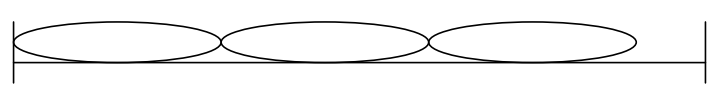
\includegraphics[scale=0.4]{images/Knezer_clique.png}
\end{center}

\underline{Оценка снизу с помощью независимых множеств}: По теореме Эрдёша-Ко-Радо \newline
$\alpha(KG_{n, k})=C^{k-1}_{n-1}$(если не разрешат использовать её, то возьмём все множества, пересекающиеся по 1, тогда получим $\alpha(KG_{n, k}) \geqslant C^{k-1}_{n-1}$), значит, по нашей оценке 
$$\chi(KG_{n, k}) \geqslant \frac{C^k_n}{C^{k-1}_{n-1}} = \frac{n}{k}$$ \\
Стоит заметить, что эта оценка почти не отличается от предыдущей, только на 1 хуже, если n не делится на k.

\underline{Простые верхние оценки}: Самая простая оценка: n. Поочерёдно будем брать множества, пересекающие по i для $i \in R_n$. Тогда каждый элемент i-го множества можно покрасить в один и тот же цвет, так как между ними нет рёбер, а всего множеств n. Эту оценку можно немного улучшить: Красим так же, как и раньше до n-k+1. Тогда неиспользованных чисел остаётся только k-1<1 для любой непокрашенной вершины, значит, это меньше, чем полноценная вершина, значит, непокрашенных вершин не осталось. Улучшенная оценка: $\chi(KG_{n, k}) \leqslant n-k+1$.

\underline{Лучшая оценка}: Повторим раскарску, но теперь до n-2k+1. Тогда все оставшиеся веришны - подмножества $R_n \setminus R_{n-2k+1}$. Тогда чисел остаётся всего 2k-1, и значит, любые две веришны пересекаются, значит, можем покрасить их в ещё один цвет и $\chi(KG_{n, k}) \leqslant n-2k+2$.

\underline{Примеры}: \\
$-$ $KG_{n, 1}=K_n$ \\
$-$ $KG_{n, k}=(V, \varnothing)$, если $k > \frac{n}{2}$ \\ 
$-$ $KG_{n, \frac{n}{2}}$ $-$ паросочетание \\
$-$ $KG_{5, 2}$ $-$ граф Петерсена

\newpage{}

\section{(5) Верхняя оценка хроматического числа кнезеровского графа. Теорема Ловаса о хроматическом числе кнезеровского графа (б/д).}
\Def Кнезеровский граф $-$ G(n, k, 0), также обозначается $KG_{n, k}$, т. е. если $R_n=\overline{1..n}$, то $V=\{ S | S \subseteq R_n\!\! \wedge\!\! |S| = k \}$ и $E=\{ (A, B) | A \in V\!\! \wedge\!\! B \in V\!\! \wedge\!\! A \cap B = \varnothing \}$.

\underline{Простые верхние оценки}: Самая простая оценка: n. Поочерёдно будем брать множества, пересекающие по i для $i \in R_n$. Тогда каждый элемент i-го множества можно покрасить в один и тот же цвет, так как между ними нет рёбер, а всего множеств n. Эту оценку можно немного улучшить: Красим так же, как и раньше до n-k+1. Тогда неиспользованных чисел остаётся только k-1<1 для любой непокрашенной вершины, значит, это меньше, чем полноценная вершина, значит, непокрашенных вершин не осталось. Улучшенная оценка: $\chi(KG_{n, k}) \leqslant n-k+1$.

\underline{Лучшая оценка}: Повторим раскарску, но теперь до n-2k+1. Тогда все оставшиеся веришны - подмножества $R_n \setminus R_{n-2k+1}$. Тогда чисел остаётся всего 2k-1, и значит, любые две веришны пересекаются, значит, можем покрасить их в ещё один цвет и $\chi(KG_{n, k}) \leqslant n-2k+2$.

\textbf{Теорема(Ловаса):} $\chi(KG_{n, k}) = n-2k+2$.
\newpage{}

\section{(8) Верхняя оценка хроматического числа кнезеровского графа. Теорема Борсука–Улама–Люстерника– Шнирельмана (б/д). Теорема Ловаса о хроматическом числе кнезеровского графа.}
\setcounter{section}{54}
\section{Матрицы Адамара. (Вторая) конструкция Пэли с квадратичными вычетами при $n = 2p + 2,p = 4m + 1$.}
\par \textbf{Утверждение (свойства кронекеровского произведения):} \begin{enumerate}
    \item $(A \otimes B)^T=A^T \otimes B^T$
    \item $(A \otimes B)(C \otimes D)=(AC) \otimes (BD)$
\end{enumerate}
\par \begin{itemize}
    \item[$\blacktriangle$ 1.] $C=A \otimes B, D = C^T$. Тогда $d_{pb+q, kb+l}=c_{kb+l, pb+q}=a_{kp} b_{lq}=(A)^T_{pk} (B)^T_{ql} \Rightarrow$ по определению $D = A^T \otimes B^T$
    \item[2.] Покажем, что это правда для случаев когда размеры $A , C$ и $B, D$ попарно равны и все матрицы квадратные. Тогда можно просто рассмотреть их произведение как блочных матриц.
    $$\left(
\begin{array}{ccc}
a_{11}B & \ldots & a_{1n}B\\
\vdots & \ddots & \vdots\\
a_{n1}B & \ldots & a_{nn}B
\end{array}
\right) \left(
\begin{array}{ccc}
c_{11}D & \ldots & c_{1n}D\\
\vdots & \ddots & \vdots\\
c_{n1}D & \ldots & c_{nn}D
\end{array}
\right)=\left(
\begin{array}{ccc}
R_{11} & \ldots & R_{1n}\\
\vdots & \ddots & \vdots\\
R_{n1} & \ldots & R_{nn}
\end{array}
\right)$$
\par где $R_{ij}=\sum_{k=1}^n (a_{ik} B)(c_{kj} D)$ (утверждение из Википедии) = $(\sum_{k=1}^n a_{ik} c_{kj})BD=(AC)_{ij} BD$ $\Rightarrow$ по определению получили $(AC) \otimes (BD) \: \blacksquare$
\end{itemize}
\par \textbf{Лемма:} \begin{enumerate}
    \item Если $p \equiv 1 (\md 4)$, то $Q_p$ - симметрична
    \item $Q_pQ_p^T=pE_p-I_p$, где $I_p$ - матрица состоящая полностью из единиц
\end{enumerate} 
\par \begin{itemize}
    \item[$\blacktriangle$ 1.] $$\left(\frac{-1}{p}\right)=(-1)^\frac{p-1}{2}=(-1)^\frac{4k}{2}=1 \Rightarrow \left(\frac{i-j}{p}\right)=\left(\frac{-1}{p}\right) \left(\frac{j-i}{p}\right)= \left(\frac{j-i}{p}\right) \Rightarrow Q_{ij}=Q_{ji}$$ 
    \item[2.] В первой конструкции Пэли мы показали, что скалярное произведение различных строк $Q_p$ равно $-1$. Скалярное произведение строк $i, j$ - это элемент на позиции $i,j$ в $Q_pQ_p^T$. Очевидно, что на диагонали будут стоять числа $p-1$, так как в каждой строке ровно $p-1$ ненулевой элемент, каждый из которых равен $\pm 1$. Таким образом, получается, что $Q_pQ_p^T=pE_p-I_p \: \blacksquare$
\end{itemize}
\par \textbf{II конструкция Пэли:} Пусть $p \equiv 1 (\md 4)$. Если в матрице
$$A=\left(
\begin{array}{cc}
0 & e^T\\
e &  Q_p
\end{array}
\right)$$
где $e$ — столбец из единиц размера $p$, $Q_p$ - матрица Якобсталя порядка $p$, заменить $0$ на матрицу 
$M_0=\left(
\begin{array}{cc}
1 & -1\\
-1 &  -1
\end{array}
\right)$, а$\; \pm 1$ на матрицу $\pm \left(
\begin{array}{cc}
1 & 1\\
1 & -1
\end{array}
\right)=\pm M_1$, то
получится матрица Адамара порядка $2p + 2$.
\par $\blacktriangle$ Найдем $AA^T$ (пригодится нам в будущем). В левом верхнем углу очевидно будет стоять $p$, так как просто перемножили столбец из единиц на строку. Остальные элементы первой строки/столбца будут нулями, так как они равны сумме всех символов Лежандра по $p$. Просто перемножая матрицы заметим, что в оставшемся пространстве у нас получится матрица $I_p+Q_pQ_p^T=I_p+pE_p-I_p=pE_p$ (по пункту 2 леммы). Таким образом, $AA^T=pE_{p+1}$
\par Пусть $H$ - матрица которая получилась после замен. Тогда так как нули находятся только на главной диагонали $$H=A \otimes M_1+E_{p+1} \otimes M_0$$
$$HH^T=(A \otimes M_1 + E_{p+1} \otimes M_0)(A \otimes M_1 + E_{p+1} \otimes M_0)^T=(A \otimes M_1 + E_{p+1} \otimes M_0)(A^T \otimes M_1^T + E_{p+1} \otimes M_0^T)$$
\par Заметим, что $M_1^T=M_1, M_0^T=M_0, M_1M_0=-M_0M_1$
$$HH^T=(A \otimes M_1)(A^T \otimes M_1)+(E_{p+1} \otimes M_0)(A^T \otimes M_1) + (A \otimes M_1)(E_{p+1} \otimes M_0) + (E_{p+1} \otimes M_0)(E_{p+1} \otimes M_0)=$$
$$=(AA^T)\otimes M_1^2 + A^T \otimes (M_0M_1) - A \otimes (M_0M_1) + E_{p+1} \otimes M_0^2$$
\par $A=A^T$ (по пункту 1 леммы), $AA^T=pE_{p+1}$. Матрицы $M_0, M_1$ являются матрицами Адамара $\Rightarrow M_i^2=M_i^TM_i=2E_2$
$$HH^T= pE_{p+1} \otimes 2E_2 + E_{p+1} \otimes 2E_2=2pE_{2p+2} + 2E_{2p+2}=(2p+2)E_{2p+2} \: \blacksquare$$
\newpage{}

\section{(8) Теорема Борсука–Улама–Люстерника–Шнирельмана: доказательство в случае замкнутых
множеств для $n = 2$ и $n = 3$.}
\setcounter{section}{55}
\section{$(n, M, d)$-коды. Граница Плоткина}
\begin{definition}
    \textit{$(n, M, d)$-кодом} называется код, в котором все кодовые слова имеют длину $n$, $d$ -- минимальное расстояние между словами (в смысле расстояния Хэмминга), $M$ -- количество кодовых слов.
\end{definition}

\begin{theorem}[Граница Плоткина]
    Пусть задан $(n, M, d)$-код. Если $2d > n$, то $M \leq \left[ \frac{2d}{2d - n} \right]$
    \begin{proof}[$\blacktriangle$]
        Пусть $\Vec{a_1}, \Vec{a_2}, ..., \Vec{a_M}$ -- все кодовые слова. Запишем их в матрицу следующим образом (каждый вектор представляется в виде строчки):
        $$\begin{pmatrix}
            \leftarrow \Vec{a_1} \rightarrow \\
            \leftarrow \Vec{a_2} \rightarrow \\
            ...\\
            \leftarrow \Vec{a_M} \rightarrow \\
        \end{pmatrix}$$
        Полученная матрица имеет размер $M \times n$.\\
        Рассмотрим сумму ($a_{i_j}$ -- элемент матрицы)
        $$
        S = \sum \limits_{k=1}^{n} \sum \limits_{1 \leq i < j \leq M} I_{ \{ a_{i_{k}} \neq a_{j_{k}} \} }, \text{где}\ I_{ \{ a_{i_{k}} \neq a_{j_{k}} \} } = 
        \begin{cases}
            1, a_{i_{k}} \neq a_{j_{k}}\\
            0, a_{i_{k}} = a_{j_{k}}
        \end{cases}
        $$
        $S$ можно рассматривать следующим образом: фиксируем столбец $k$ и смотрим количество несовпадающих пар в этом столбце. Пусть $x$ -- число единиц в этом столбце, тогда $M - x$ -- число нулей в этом же столбце. Тогда несовпадающих пар в этом столбце ровно $x(M-x) = Mx - x^2$. Максимум этого значения достигается при $x = \frac{M}{2}$, то есть $x(M-x) \leq \frac{M^2}{4}$. Получаем, что $S \leq n \cdot \frac{M^2}{4}$.\\
        Теперь рассмотрим $S$ с другой стороны, переставив знаки суммирования:\\
        $$
        S = \sum \limits_{1 \leq i < j \leq M} \sum \limits_{k=1}^{n} I_{ \{ a_{i_{k}} \neq a_{j_{k}} \} }
        $$
        Теперь $S$ можно интерпретировать следующим образом: зафиксируем строки $i$ и $j$ (а значит, и соответствующие кодовые слова $\Vec{a_i}$ и $\Vec{a_j}$). Тогда внутренняя сумма $\sum \limits_{k=1}^{n} I_{ \{ a_{i_{k}} \neq a_{j_{k}} \} }$ -- это в точности расстояние Хэмминга $d(\Vec{a_i}, \Vec{a_j})$. По определению $(n, M, d)$-кода $d(\Vec{a_i}, \Vec{a_j}) \geq d$, то есть $S \geq \frac{M(M-1)}{2} \cdot d$, где ($\frac{M(M-1)}{2}$ -- количество пар $(i, j)$).\\
        $$
            \frac{M(M-1)}{2} \cdot d \leq S \leq n \cdot \frac{M^2}{4}
        $$
        $$
            (M - 1)d \leq n \cdot \frac{M}{2}
        $$
        $$
            dM - \frac{nM}{2} \leq d
        $$
        $$
            M(d - \frac{n}{2}) \leq d
        $$
        $$
            M(2d - n) \leq 2d
        $$
        Так как $2d - n$ -- положительное, то можно разделить на него
        $$
            M \leq \frac{2d}{2d - n}
        $$
        Так как $M$ -- натуральное, получаем:
        $$
            M \leq \left[ \frac{2d}{2d - n} \right]
        $$
    \end{proof}
\end{theorem}
\newpage{}

\section{(6) Максимальное число $m(n, k, t)$ подмножеств $n$-элементного множества, в каждом из которых ровно $k$ элементов и среди которых любые два множества пересекаются не по $t$ элементам. Точное значение для $m(n, 3, 1)$: явная конструкция и оценка по индукции. Линейно-алгебраическая оценка для $m(n, 3, 1)$.}
\textbf{Определение.}
$$
m(n, r, s) := max \{ k : \exists r \text{-однородный гиперграф на } n \text{ вершинах } :
|E| = k \text{ и } \forall A, B \in E \ |A \cap B| \neq s \}
$$

Другая интерпретация:

$m(n, r, s)$ -- максимальное число подмножеств $n$-элементного множества, в каждом из
которых ровно $r$ элементов и среди которых любые два множества пересекаются не по $s$
элементам.

\textbf{Явная конструкция для $m(n, 3, 1)$}

Рассмотрим граф $G(n) = (V, E)$, где 
$V = \{ A \subset \{1, 2, \ldots, n\} : |A| = 3\}$ ($|V| = C_n^3$), а

$E = \{ (A, B)\ :\ |A \cap B| = 1\}$.

Тогда $m(n, 3, 1) = \alpha(G(n))$.

Утверждается, что

\begin{equation*}
\alpha(G(n)) = 
\begin{cases}
n & \text{если } n \equiv 0 \pmod 4\\
n - 1 & \text{если } n \equiv 1 \pmod 4\\
n - 2 & \text{иначе}
\end{cases}
\end{equation*}

Оставлено в качестве упражнения. 
Доказательство можно провести индукцией по $n$ (если успею, допишу).

\textbf{Линейно-алгебраическая оценка для $m(n, 3, 1)$}

$$
m(n, 3, 1) = \alpha(G(n)) \leq n
$$

\textit{Доказательство.}
Пусть $W \subset V$ -- независимое множество вершин,
$W = \{ A_1, \ldots, A_t \}$.

$$
\forall i\ |A_i| = 3; \forall i \neq j |A_i \cap A_j| \in \{0, 2\}
$$

Каждому $A_i$ сопоставим вектор $\overline{x_i} = (x^1, \ldots, x^n) \in \mathbb{Z}_2^n$,
в котором $x^j = 1 \Leftrightarrow j \in A_i$.
Тогда мощность пересечения $A_i$ и $A_j$ выражается как скалярное произведение $\overline{x_i}$ и $\overline{x_j}$:
$|A_i \cap A_j| = (\overline{x_i}, \overline{x_j})$.

Докажем, что $\overline{x_1}, \ldots, \overline{x_t}$ 
линейно независимы над $\mathbb{Z}_2^n$.

Пусть $c_1 \overline{x_1} + \ldots + c_t \overline{x_t} = \overline{0}$. Левую и правую часть равенство скалярно умножим на $x_1$ в $\mathbb{Z}_2^n$:

$$
    c_1 \underbrace{(\overline{x_1}, \overline{x_1})}_{\equiv 1} + 
    c_2 \underbrace{(\overline{x_1}, \overline{x_2})}_{\equiv 0} + \ldots +
    c_t \underbrace{(\overline{x_1}, \overline{x_t})}_{\equiv 0} = 0
$$

Получается, $c_1 = 0$. Аналогично $c_2 = c_3 = \ldots = c_t = 0$.

Это означает, что $\overline{x_1}, \ldots, \overline{x_t}$ независимы в $\mathbb{Z}_2^n$, а значит $t \leqslant dim \mathbb{Z}_2^n = n$.
\newpage{}

\section{(6) Величина $m(n, k, t)$. Линейно-алгебраическая оценка для $m(n, 3, 1)$ (б/д). Аналогичная оценка для $m(n, 5, 2)$ и ее асимптотическая неулучшаемость.}
\textbf{Определение.}
$$
m(n, r, s) := max \{ k : \exists r \text{-однородный гиперграф на } n \text{ вершинах } :
|E| = k \text{ и } \forall A, B \in E \ |A \cap B| \neq s \}
$$

Другая интерпретация:

$m(n, r, s)$ -- максимальное число подмножеств $n$-элементного множества, в каждом из
которых ровно $r$ элементов и среди которых любые два множества пересекаются не по $s$
элементам.

Можно ввести граф $G(n, r, s)$, у которого
$V = \{ A \subset \{1, 2, \ldots, n\} : |A| = r \}$,
$E = \{ (A, B) : |A \cap B| = s \}$.
Тогда $m(n, r, s) = \alpha(G(n, r, s))$.

\textbf{Линейно-алгебраическая оценка для $m(n, 3, 1)$.}

$$
m(n, 3, 1) \leq n
$$

\textbf{Линейно-алгебраическая оценка для $m(n, 5, 2)$ и её асимптотическая неулучшаемость.}

Можно легко получить нижнюю оценку на $m(n, 5, 2)$: зафиксируем первые три элемента, а остальные два произвольно выберем из оставшихся. Тогда получившиеся множества будут пересекаться как минимум по трём элементам. Получается, 

$$
m(n, 5, 2) \geqslant C_{n - 3}^2 \sim \frac{n^2}{2}
$$

Из следующей теоремы видно, что оценки нельзя улучщить асимптотически.

\textbf{Теорема.}

$$
m(n, 5, 2) \leqslant C_n^2 + 2C_n^1 + C_n^0 \sim \frac{n^2}{2}
$$

\textit{Доказательство.}

Пусть $H = (V, E)$. Каждому ребру $A \in E$ сопоставим вектор
$\overline{x_A} = (x^1, \ldots, x^n)$, где $x^j = 1 \Leftrightarrow j \in A$.

Пусть $\{ \overline{x_1}, \ldots \overline{x_t} \}$ -- все векторы, построенные 
по рёбрам гиперграфа.
Каждому вектору $\overline{x_i}$ сопоставим 
формальный многочлен $P_{\overline{x_i}} \in \mathbb{Z}_3 [y_1, \ldots, y_n]$.

$$
P_{\overline{x_i}} = (\overline{x_i}, \overline{y}) \cdot 
((\overline{x_i}, \overline{y}) - 1), \text{ где } \overline{y} = (y_1, \ldots, y_n).
$$

\textit{Пример для понимания}

Если $A = \{1, 2, 4, 5, 8\}$, то 
$\overline{x_A} = (1, 1, 0, 1, 1, 0, 0, 1, 0 \ldots, 0)$, а

$P_{\overline{x_A}}(\overline{y}) = 
(y_1 + y_2 + y_4 + y_5 + y_8) (y_1 + y_2 + y_4 + y_5 + y_8 - 1)$.
\\

Докажем, что $P_{\overline{x_1}}, \ldots, P_{\overline{x_t}}$ линейно независимы над $\mathbb{Z}_3$.

$$
c_1 P_{\overline{x_1}} + \ldots + c_t P_{\overline{x_t}} = 0
\Rightarrow
\forall \overline{y} \in \{ 0, 1 \}^n \ 
c_1 P_{\overline{x_1}}(\overline{y}) + \ldots + c_t P_{\overline{x_t}}(\overline{y}) = 0
$$

Возьмём $\overline{y} = \overline{x_1}$.

$P_{\overline{x_1}}(\overline{x_1}) = 
(\overline{x_1}, \overline{x_1})((\overline{x_1}, \overline{x_1}) - 1) = 
5 \cdot (5 - 1) = 20 \equiv 2 \pmod{3}$.

Для $i \geqslant 2$:

$P_{\overline{x_i}}(\overline{x_1}) = 
(\overline{x_i}, \overline{x_1})((\overline{x_i}, \overline{x_1}) - 1)$.

$(\overline{x_i}, \overline{x_1}) = |A_1 \cap A_i|$. 
Возможные значения $|A_1 \cap A_i|$: 0, 1, 3, 4. По модулю 3 это только 0 и 1.
Видно, что если вместо скалярного произведения мы подставим 0 или 1, то 
$P_{\overline{x_i}}(\overline{x_1}) = 0$.

Из этого следует, что $c_1 = 0$. Аналогично $c_2 = \ldots = c_t = 0$. 
Поэтому $P_{\overline{x_1}}, \ldots, P_{\overline{x_t}}$ линейно независимы над $\mathbb{Z}_3$, а значит $t \leqslant dim \mathbb{Z}_3 [y_1, \ldots, y_n]$.

Какова же размерность пространства $\mathbb{Z}_3 [y_1, \ldots, y_n]$? 
Очевидно, это количество базисных векторов. 
Базисные векторы в $\mathbb{Z}_3 [y_1, \ldots, y_n]$ 
(с учётом того, что все наши многочлены степени не выше 2):

$y_i y_j, i \neq j$ -- их $C_n^2$.

$y_i^2, i = 1, \ldots, n$ -- их $C_n^1$

$y_i, i = 1, \ldots, n$ -- их $C_n^1$

$1$ -- $C_n^0$

Получилось, что $t \leqslant C_n^2 + 2C_n^1 + C_n^0$.
\newpage{}

\section{(7) Общая теорема Франкла–Уилсона для $m(n, k, k - p)$ при $k < 2p$.}

\Th $r < 2p, s = r - p$, $p$~--- простое, тогда $m(n, r, s) \leq \sum\limits_{k = 0}^{p - 1}C_n^k$

\Proof Рассмотрим множество:

$$
E = \{A_1, \ldots, A_t \ | \ |A_i| = r, \ |A_i \bigcap A_j| \ne s\},
$$ 

где $\forall i: A_i$ -- подмножество нашего $n$-элементного множества.

Каждому множеству $A_i$ можно сопоставить $n$-мерный вектор $x_i$, состоящий из ноликов и единичек ($1$ -- элемент есть, $0$ -- нет).

Тогда множество $E$ можно переписать в следующем виде:

$E = \{x_1, \ldots, x_t \ | x_i \in \{0, 1\}^n, \ x_i^1 + \ldots + x_i^n = r, \ (x_i, x_j) \ne s\}$, где $x_i^j$ -- $j$-ая координата вектора $x_i$

Теперь введем многочлены для $x_i$:
$P_{x_i} \in \mathbb{Z}_p[y_1, \ldots, y_n]$, 

$$P_{x_i}(y) = \prod_{j = 0, \ j \not\equiv s (p)}^{p - 1}(j - (x_i, y))$$.

Далее введем многочлены $P'_{x_i}(y)$, которые получаются из многочленов $P_{x_i}(y)$ <<срезанием>> степени и приведением подобных. (То есть все степени больше единицы у $y_i$ станут равными единице, что не меняет значения многочлена, так как $x_i^k, y_i \in \{0, 1\}$).

Тогда покажем, что многочлены вида $P'$ задают базис, то есть линейно независимы, а всего их $\sum\limits_{k = 0}^{p - 1}C_n^k$.

$$
c_1 P'_{x_1} + \ldots + c_t P'_{x_t} = 0 \Longrightarrow \forall y \in \{0, 1\}^n \ c_1 P'_{x_1}(y) + \ldots + c_t P'_{x_t}(y) \equiv 0 \ (mod \ p) \Longrightarrow
$$

$$
c_1 P_{x_1} + \ldots + c_t P_{x_t} = 0 \Longrightarrow \forall y \in \{0, 1\}^n \ c_1 P_{x_1}(y) + \ldots + c_t P_{x_t}(y) \equiv 0 \ (mod \ p)
$$

Теперь рассмотрим\\

$P_{x_i}(x_i) = \prod\limits_{j = 0, \ j \not\equiv s (p)}^{p - 1}(j - (x_i, x_i)) \not\equiv 0 \ (mod \ p),$ т.к. $(x_i, x_i) = r$\

$\ P_{x_i}(x_j) = \prod\limits_{j = 0, \ j \not\equiv s (p)}^{p - 1}(j - (x_i, x_j)) \equiv 0 \ (mod \ p)
$

Последнее сравнение по модулю верно, так как $(x_i, x_j) < r, (x_i, x_j) \ne s, r, s - \ell p, \ell \in \mathbb{N}$ (для разности верно, так как $r < 2p$), то есть $(x_i, x_j)$ не сравнимо с $s$ по модулю $p$.

Тогда найдется скобка в произведении в определении многочлена, для которой $j \equiv (x_i, x_j) \ (mod \ p)$. Тогда

$$\forall i \ P_{x_1}(x_i) + \ldots + c_t P_{x_t}(x_i) \equiv P_{x_i}(x_i)c_i \ (mod \ p) \Longrightarrow P_{x_i}(x_i)c_i \equiv 0 \ (mod \ p) \Longrightarrow c_i \equiv 0 \ (mod \ p)$$ 

(Т.к. $P_{x_i}(x_i) \not\equiv 0 \ (mod \ p)$)

Все переходы верны в силу простоты $p$, а значит было получено, что эти одночлены $P'_{x_i}$ действительно линейно независимы, а значит задают базис. Таким образом, теорема доказана.

\EndProof

\newpage{}

\section{(9) Теорема Франкла–Уилсона для $m(n, k, k - p)$ при $k \geqslant 2p$.}

\Th Пусть $r - s = p$, $p$ -- простое. Пусть $r - 2p \geq 0$, $d := r - 2p + 1 = 2s - r + 1$

Тогда $m(n, r, s) \le \frac{C_n^d}{C_r^d} \sum\limits_{k=0}^{p-1}C_{n-d}^k$

\Proof

$\{1, 2, \ldots, n\}$ -- вершины гиперграфа $H = (V, E)$, $H - r$-однороден и $\forall A, B \in E |A \cap B| \neq s$

$E = \{A_1, \ldots, A_t\}$ -- ребра. Наша цель доказать, что $t$ не больше, чем та страшная оценка сверху в формулировке теоремы.

Рассмотрим $D_1, \ldots, D_{C_n^d}$ -- все возможные $d-$элементные подмножества в $V$.\\

\textit{Идейно наша цель на будущее:} доказать, что среди них есть множество вершин, которые задействованы в большом количестве ребер. Тогда их можно будет удалить и запустить линейно-алгебраический метод.\\

Определим $I(A_i, D_j) = 
 \begin{cases}
   1, & D_j \subset A_i\\
   0, &\text{иначе}
 \end{cases}$
 
Просуммируем индикатор двумя способами:
$\sum\limits_{i=1}^t \sum\limits_{j=1}^{C_n^d} I(A_i, D_j) = 
\sum\limits_{j=1}^{C_n^d} \sum\limits_{i=1}^t I(A_i, D_j)$

$\sum\limits_{i=1}^t \sum\limits_{j=1}^{C_n^d} I(A_i, D_j) = \sum\limits_{i=1}^t C_r^d = tC_r^d$, тогда $\exists j : \sum\limits_{i=1}^t I(A_i, D_j) \ge \frac{tC_r^d}{C_n^d}$

То есть мы нашли множество вершин $D_j$, которое содержится не менее, чем в $\frac{tC_r^d}{C_n^d}$ ребрах. Пусть это ребра $A'_1, \ldots, A'_{\tau}$. При этом, мы знаем, что $t \le \frac{C_n^d}{C_r^d}\tau$.

\textit{Цель:} $\tau \le \sum\limits_{k=0}^{p-1}C_{n-d}^k$\\

Без ограничения общности будем считать, что $D_j = \{1, \ldots, d\}$. Перейдем от множеств $A'_i$ к векторам $\overline{x_i}$, где $1$ стоит на месте элемента, который есть в множестве, $0$ -- на месте элемента, которого нет в множестве. Заметим, что у всех таких векторов на первых $d$ позициях стоят $1$.

$P_{\overline{x_i}}(\overline{y}) = \prod\limits_{j = 0, \ j \not\equiv s (p)}^{p - 1}(j - (\overline{x_i}, \overline{y})) \to P'_{\overline{x_i}}(\overline{y})$ (срезаем степени)

$P_{\overline{x_i}} \in \mathbb{Z}_p[y_{d+1}, \ldots, y_n]$, $\overline{y} = (1, \dots, 1, y_{d+1}, \ldots, y_n)$

Размерность $P'_{\overline{x_i}}$ равна $\sum\limits_{k=0}^k$ (т.к. сократили степени), осталось доказать линейную независимость.

$c_1P'_{\overline{x_1}} + \ldots + c_{\tau}P'_{\overline{x_{\tau}}} = 0$

$\forall y \in \{\overline{x_1}, \ldots, \overline{x_{\tau}}\} : c_1P'_{\overline{x_1}}(\overline{y}) + \ldots + c_{\tau}P'_{\overline{x_{\tau}}}(\overline{y}) = 0$

Подставим $\overline{y} = \overline{x_i}$, тогда $P(\overline{x_i})(\overline{x_i}) \neq 0(p)$ (т.к. $(\overline{x_i}, \overline{x_i}) = r$)

$r - 2p + 1 = d \le (\overline{x_i}, \overline{x_j}) \le r$, и при этом $(\overline{x_i}, \overline{x_j}) \neq r-p$, поэтому $(\overline{x_i}, \overline{x_j}) \neq r(p)$, и $P_{\overline{x_j}}(\overline{x_i}) = 0(p)$

Тогда $c_i = 0 \ \forall i$, ЛНЗ доказана

\EndProof
\newpage{}

\section{(8) Точность обеих теорем Франкла–Уилсона при постоянных $k, t$. Максимальное число $k$-элементных подмножеств $n$-элементного множества, из которых любые два множества пересекаются не более чем по $t$ элементам. Связь с теорией кодирования, теорема Рёдля (б/д).}

\Def $h(n, r, s) - max \ k$, что $\exists r$-однородный гиперграф $H = (V, E), |V| = n, |E| = k, \forall A, B \in E \ |A \cap B| \leq s$

На самом деле, $h(n, r, s)$ -- задача теории кодирования. А именно, мы каждому ребру сопоставим вектор из $0$ и $1$ ($1$ -- элемент есть, $0$ -- нет). Тогда в теории кодирования можно рассмотреть такую задачу: мы кодируем слова такими векторами из $0$ и $1$ (всего единиц $r$ штук в каждом из них). Далее мы посимвольно передаем какое-то слово по зашумленному каналу связи. В итоге у нас могут получиться ошибки -- какие-то символы прочитались неправильно. Известно, что таких ошибок не более $d$. Тогда вопрос, какое максимальное количество слов можно <<уметь распознавать>>, чтобы по полученному слову однозначно понять, какое слово передавалось. То есть мы хотим, чтобы у любых двух возможных слов общая часть была размера не более, чем $r-d$. Обозначим $r-d-1$ за $s$ и получим в точности задачу для поиска $h(n, r, s)$

\Th $h(n, r, s) \leq \frac{C_n^{s+1}}{C_r^{s+1}}$

\Proof
$H = (V, E), |V|=n, |E|=k, \forall A, B \in E \ |A\cap B| \leq s, |A| = |B| = r$

Рассмотрим все $(s+1)$-элементные подмножества $V$. Их $C_n^{s+1}$

$F = {A_1, \ldots, A_k}$, в ребро $A_i$ попадает $C_r^{s+1}$ подмножеств мощности $(s+1)$, а ребра не пересекаются по $(s+1)$-элементным подмножествам.
\EndProof\\

\Th (Рёдля) $h(n, r, s) \geq (1 + o(1))\frac{C_n^{s+1}}{C_r^{s+1}}$ при фикс. $r, s$ и $n \to \infty$

\textbf{1) Асимптотика первой теоремы (когда $r - 2p < 0$)} при фиксированных $r, s$ и $n \to \infty$

Хотим доказать: $m(n,r,s) \geq C_{n-s-1}^{r-s-1} \sim \frac{n^{r-s-1}}{(r-s-1)!}$

Построим пример:

Рассмотрим множество из $n$ элементов.

Возьмем первые $s + 1$ элемент и скажем, что они присутствуют во всех $r$-элементных множествах, которые мы хотим построить. Тогда оставшиеся $r-s-1$ элемент мы будем выбирать из $n-s-1$ возможных. Тогда таким образом мы можем построить как раз $C_{n-s-1}^{r-s-1}$ множеств, которые пересекаются по $s+1$ элементу. 

Мы получили оценку снизу с той же асимптотикой, что и для оценки сверху, значит, оценка асимптотически не улучшается (то есть точна).

\textbf{2) Асимптотика второй теоремы (когда $r - 2p \geq 0$)} при фиксированных $r, s$ и  $n \to \infty$

$C_n^d \sim \frac{n^d}{d!} = \frac{n^{2s-r+1}}{(2s-r+1)!}$

$C_r^d = \frac{r!}{(2s-r+1)!(2r-2s-1)!}$

$\frac{C_n^d}{C_r^d} \sim \frac{n^{2s-r+1}(2r-2s-1)!}{r!}$

$C_{n-d}^k \sim \frac{n^k}{k!} \Rightarrow \sum\limits_{k=0}^{p-1}C_{n-d}^k \sim C_{n-d}^{p-1} \sim \frac{n^{r-s-1}}{(r-s-1)!}$

$\frac{C_n^d}{C_r^d}\sum\limits_{k=0}^{p-1}C_{n-d}^k \sim n^s\frac{(2r-2s-1)!}{r!(r-s-1)!}$

\textbf{Теперь построим конструкцию для оценки снизу}, у которой будет точно такая же асимптотика.

Нам нужно построить как можно больше ребер мощности $r$, никакие два из которых не пересекаются по $s$ вершинам.

Пусть $a = 2r-s-1$. Тогда среди $a$ элементов любые два $r$-элементных подмножества будут пересекаться хотя бы по $s+1$ элементу. Всего ребер на этих $a$ элементах $C_{2r-s-1}^r$.

Найдем как можно больше $a$-элементных множеств (подмножеств множества вершин), что каждые два из них пересекаются по $\le s-1$ элементам. Это ровно задача из теории кодирования (код, исправляющий ошибки). Количество таких элементов мы обозначали как $h(n, a, s-1)$.

По двум теоремам из начала билета $h(n, a, s-1) \sim \frac{C_n^s}{C_a^s}$.

Положим $h = h(n, a, s-1)$, тогда $A_1, \ldots, A_h : \forall i \ |A_i| = a, |A_i\cap A_j| \leq s-1$.

В каждом $A_i$ возьмем все $r$-элементные множества. Между собой они пересекаются хотя бы по $s+1$ элементу. А множества из разных $A$ пересекаются не более, чем по $s-1$ элементу. Значит, мы построили $hC_{2r-s-1}^r$ множеств мощности $r$.

$hC_{2r-s-1}^r \sim \frac{C_n^s}{C_{2r-s-1}}^sC_{2r-s-1}^r \sim
\frac{n^s}{s!}\frac{(2r-s-1)!}{r!(r-s-1)!}\frac{s!(2r-2s-1)!}{(2r-s-1)!} = n^s\frac{(2r-2s-1)!}{r!(r-s-1)!}$

Значит, оценка асимптотически не улучшается.
\newpage{}

\section{(6) Задача об уклонении: верхняя оценка уклонения величиной 
$\sqrt{2n \ln (2s)}$ с доказательством и величиной $6 \sqrt{n}$ б/д.}
\textbf{Задача об уклонении}

Пусть задан гиперграф с множеством вершин $V = \{ 1, \ldots, n \}$ и множеством рёбер
$\mathcal{M} = \{ M_1, \ldots, M_m \}$ (гиперграф не обязательно однородный). 
Также $\mathcal{M}$ можно интерпретировать как набор подмножеств 
множества $\{1, \ldots, n \}$.

Пусть $\chi$ -- раскраска вершин в два цвета:
$\chi: \{1, \ldots, n \} \to \{ -1, 1 \}$.

Введём функцию $\chi(M_i) := \sum \limits_{j \in M_i} \chi(j)$. 
Эта функция показывает "неравномерность" покраски ребра $M_i$. 
Также введём функцию разброса 
$disc(\mathcal{M}, \chi) := \max \limits_{M_i \in \mathcal{M}} \left| \chi(M_i) \right|$.
Она показывает "неравномерность" покраски в целом (максимальная "неравномерность" покраски ребра). 
Функция $disc(\mathcal{M}) := \min \limits_{\chi} disc(\mathcal{M}, \chi)$ 
минимизирует "неравномерность" раскраски.

\textbf{Теорема (б/д).}

$$
\forall n \forall \mathcal{M} = \{ M_1, \ldots, M_n \} \ 
disc(\mathcal{M}) \leqslant 6 \sqrt{n}
$$

\textbf{Теорема.}

$$
\forall \mathcal{M} = \{ M_1, \ldots, M_m \} \ 
disc(\mathcal{M}) \leqslant \sqrt{2n \ln (2m)}
$$

\textit{Доказательство.}

Рассмотрим случайную раскраску $\chi$ 
(каждой вершине независимо присвоим цвет $1$ или $-1$ с вероятностью $\frac{1}{2}$).

Можно заметить, что $\chi(M_i)$ -- сумма независимых случайных величин, 
принимающих значения $\pm 1$ с вероятностью $\frac{1}{2}$.
Значит $\chi(M_i)$ можно интерпретировать как случайное блуждание ($k := |M_i|$):
$$
P \left( \left| \chi(M_i) \right| \geqslant a \right) \leqslant
2 e^{-\frac{a^2}{2k}} \leqslant 2 e^{-\frac{a^2}{2n}}
$$

Двойка перед $e^{-\frac{a^2}{2k}}$ появилась из-за модуля. 
Возьмём $a := \sqrt{2n \ln (2m)}$:

$$
P \left( \left| \chi(M_i) \right| \geqslant a \right) \leqslant 
2 e^{-\frac{2n \ln (2m)}{2n}} = \frac{2}{2m} = \frac{1}{m}
$$

Значит, 

$$
P \left( \exists i : \left| \chi(M_i) \right| \geqslant a \right) <
m \cdot \frac{1}{m} = 1 \Rightarrow
P \left( \forall i : \left| \chi(M_i) \right| < a \right) > 0
$$
\newpage{}

\section{(6) Энтропия. Свойство полуаддитивности.}
Пусть $X$ -- случайная величина, $X: \Omega \to S \subset \mathbb{R}, |S| < \infty$.

\textit{Энтропией} случайной величины $X$ называется
$H(X) := - \sum \limits_{s \in S} P(X = s) \cdot \log_2 P(X = s)$.

Аналогично определяется энтропия для нескольких случайных величин:

$$
H(X_1, \ldots, X_n) := \sum_{s_1 \in S_1} \ldots \sum_{s_n \in S_n} 
P(X_1 = s_1, \ldots, X_n = s_n) \cdot \log_2 P(X_1 = s_1, \ldots, X_n = s_n)
$$

\textbf{Теорема (свойство полуаддитивности).}

$$
H(X, Y) \leqslant H(X) + H(Y)
$$

\textit{Доказательство.}

Пусть $X: \Omega \to S, Y: \Omega \to T$.

Докажем, что $H(X) + H(Y) - H(X, Y) \geqslant 0$.

\begin{multline*}
H(X) + H(Y) - H(X, Y) = 
- \sum_{s \in S} P(X = s) \cdot \log_2 P(X = s)
- \sum_{t \in T} P(Y = t) \cdot \log_2 P(Y = t) + \\
+ \sum_{s \in S} \sum_{t \in T} P(X = s, Y = t) \cdot \log_2 P(X = s, Y = t) = 
- \sum_{s \in S} \left( \left( \sum_{t \in T} P(X = s, Y = t) \right) 
\cdot \log_2 P(X = s) \right) - \\
- \sum_{t \in T} \left( \left( \sum_{s \in S} P(Y = t, X = s) \right) 
\cdot \log_2 P(Y = t) \right)
+ \sum_{s \in S} \sum_{t \in T} P(X = s, Y = t) \cdot \log_2 P(X = s, Y = t) = \\
= \sum_{s \in S} \sum_{t \in T} P(X = s, Y = t) \cdot 
\log_2 \frac{P(X = S, Y = t)}{P(X = s) P(Y = t)} = \\
= \sum_{s \in S} \sum_{t \in T} 
\underbrace{\frac{P(X = s, Y = t)}{P(X = s) P(Y = t)}}_{z_{s, t}} \cdot 
P(X = s) P(Y = t) \cdot 
\log_2 \underbrace{\frac{P(X = S, Y = t)}{P(X = s) P(Y = t)}}_{z_{s, t}} = \\
= \sum_{s \in S} \sum_{t \in T} z_{s, t} \cdot \log_2 z_{s, t} \cdot P(X = s) P(Y = t)
\end{multline*}

Так как функция $f(x) = x \log_2 x$ выпуклая, то можно воспользоваться неравенством Йенсена:

\begin{multline*}
\sum_{s \in S} \sum_{t \in T} f(z_{s, t}) \cdot P(X = s) P(Y = t) \geqslant
f \left( \sum_{s \in S} \sum_{t \in T} P(X = s) P(Y = t) \cdot z_{s, t} \right) = \\
 = f \left( \sum_{s \in S} \sum_{t \in T} P(X = s, Y = t) \right) = f(1) = 0
\end{multline*}
\newpage{}

\section{(10) Задача об уклонении. Верхняя оценка уклонения величиной $O(\sqrt{n})$: 
лемма Клейтмана б/д, шаги раскраски на недокрашенной части б/д, 
остальное -- с доказательством.}
\newpage{}

\section{(4) Задача о наименьшем числе рёбер в $n$-однородном гиперграфе с хроматическим числом хотя бы три. 
Верхняя оценка величиной $C_{2n - 1}^n$ и нижняя оценка величиной $2^{n - 1}$.}
Введём такое обозначение:
$$
m(n) = \min \{ k : \exists n-\text{однородный гиперграф } H \text{ с } 
k \text{ рёбрами и } \chi(H) > 2 \} 
$$

Напомним, что $\chi(H)$ -- минимальное количество цветов, в которое можно покрасить вершины гиперграфа так, чтобы ни одно ребро не было одноцветным.

\textbf{Теорема 1.}

$$
    m(n) \geqslant 2^{n - 1}
$$

\textit{Доказательство.}

Чтобы доказать это неравенство нужно показать, что для любого гиперграфа $H$ с количеством рёбер $k < 2^{n - 1}$ $\chi(H) \leqslant 2$. Докажем, что такой гиперграф можно раскрасить в 2 цвета правильным образом.

Пусть $A_i$ -- событие, которое состоит в том, что $i$-е ребро одноцветно.
$$
    P(A_i) = 2 \cdot \frac{1}{2^n} = 2^{1 - n} \\
$$

$$
P \left( \bigcup_{i = 1}^{k} A_i \right) \leqslant k \cdot P(A_i) < 
    2^{n - 1} \cdot 2^{1 - n} = 1
$$

$$
P \left( \bigcap_{i = 1}^{k} \overline{A_i} \right) > 0
$$

Это означает, что правильная раскраска из двух цветов существует и $\chi(H) \leqslant 2$.

\textbf{Теорема 2.}

$$
    m(n) \leqslant C_{2n - 1}^{n}
$$

\textit{Доказательство.}

Чтобы доказать это неравенство нужно показать, что существует $n$-однородный гиперграф с
$C_{2n - 1}^{n}$ рёбрами, который нельзя раскрасить в 2 цвета правильным образом.

Возьмём гиперграф с $2n - 1$ вершинами со всеми возможными рёбрами (то есть полный $n$-однородный гиперграф с $2n - 1$ вершинами). Если мы $2n - 1$ вершину покрасим в два цвета, то по принципу Дирихле найдутся $n$ вершин, покрашенных в один цвет. Так как наш граф полный, то эти $n$ вершин образуют ребро, а значит оно получилось одноцветным. 
\newpage{}

\section{(7) Задача о наименьшем числе рёбер в $n$-однородном гиперграфе с хроматическим числом хотя бы три. Верхняя оценка величиной $\frac{e \ln2}{4} n^2 2^n (1 + o(1))$.}
\textbf{Теорема 3.}

$$
m(n) \leqslant (1 + o(1)) \frac{e \ln 2}{4} n^2 2^n
$$

\textit{Доказательство.}

В дальнейшем будем считать, что $n$ -- чётно. Случай с нечётным $n$ аналогичный.

Определим множество вершин нашего гиперграфа таким образом:
$V = \{1, 2, \dots, v\}$, где $v = \frac{n^2}{2}$.

Пусть $m$ -- количество рёбер в гиперграфе. (Цель: доказать, что $m \sim \frac{e \ln 2}{4} n^2 2^n$).

Построим случайный гиперграф: выбираем рёбра с возвращением (согласно классическому определению вероятности). Если некоторые рёбра мы выберем несколько раз, то просто их отождествим.

Пусть $A_i$ -- событие, что мы выбрали $i$-е ребро. Тогда $P(A_i) = \frac{1}{C_v^n}$.

Зафиксируем конкретную раскраску $\chi$ множества вершин в 2 цвета (всего их $2^v$). Пусть в этой раскраске $r$ вершин красного цвета и $b$ -- синего ($r + b = v$).

$$
P(A_1 \text{ одноцветно в } \chi) = \frac{C_r^n + C_b^n}{C_v^n} \geqslant 
\frac{2 C_{\frac{v}{2}}^n}{C_v^n} := p
$$

Здесь мы воспользовались выпуклостью биномиального коэффициента (это свойство было при доказательстве оценок для двудольных чисел Рамсея) и обозначили получившуюся дробь за $p$ (которая, кстати, не зависит от раскраски $\chi$).

$$
P(A_1 \text{ неодноцветно в } \chi) \leqslant 1 - p
$$
Всего у нас $m$ рёбер, поэтому
$$
P(\forall i \ A_i \text{ неодноцветно в } \chi) \leqslant (1 - p)^m
$$
$$
P(\exists \chi \ :\  \forall i \ A_i \text{ неодноцветно в } \chi) \leqslant
2^v (1 - p)^m < 1
$$
$$
P(\forall \chi \  \exists i \ :\ A_i \text{ одноцветно в } \chi) \geqslant
1 - 2^v (1 - p)^m
$$
Если $1 - 2^v (1 - p)^m > 0$, то в любой раскраске есть одноцветное ребро. Теперь распишем это неравенство:

\begin{multline*}
C_v^n = \frac{v (v - 1) \ldots (v - n + 1}{n!} = 
\frac{v^n}{n!} \left( 1 - \frac{1}{v} \right) \ldots \left( 1 - \frac{n - 1}{v} \right) = \\
= \frac{v^n}{n!} e^{-\frac{1}{v} - \ldots - \frac{n - 1}{v} + 
O \left( \frac{1}{v^2} + \ldots + \frac{(n - 1)^2}{v^2} \right)}
= \frac{v^n}{n!} e^{-\frac{n(n - 1)}{2v} + O \left( \frac{n^3}{v^2} \right)}
\end{multline*}

Так как $v = \frac{n^2}{2}$, то $O \left( \frac{n^3}{v^2} \right) = O \left( \frac{1}{n} \right) \to 0, n \to \infty$.

$$
\frac{v^n}{n!} e^{-\frac{n(n - 1)}{2v} + O \left( \frac{n^3}{v^2} \right)}
\sim \frac{v^n}{n!} \cdot e^{-\frac{n^2}{2v} + \frac{n}{2v}}
$$

Так как $v = \frac{n^2}{2}$, то $\frac{n}{2v} \to 0, n \to \infty$. Поэтому

$$
\frac{v^n}{n!} \cdot e^{-\frac{n^2}{2v} + \frac{n}{2v}} \sim
\frac{v^n}{n!} \cdot e^{-\frac{n^2}{2v}} \sim
\frac{v^n}{n!} e^{-1}
$$

Аналогично 

$$
C_{\frac{v}{2}}^{n} \sim \frac{\left( \frac{v}{2} \right)^n}{n!} e^{-2}
$$

Поэтому

$$
p = \frac{2 C_{\frac{v}{2}}^n}{C_v^n} \sim 2^{1 - n} \cdot e^{-1}
$$

$$
2^v \cdot (1 - p)^m \leqslant 2^v \cdot e^{-pm} = 
e^{\frac{n^2}{2} \cdot \ln 2 - 2^{1 - n} \cdot e^{-1} \cdot m}
$$

Так как $m \sim (1 + o(1))\frac{e \ln 2}{4} n^2 2^n$, то

$$
2^{1 - n} \cdot e^{-1} \cdot m \sim
(1 + o(1)) 2^{1 - n} \cdot e^{-1} \cdot \frac{e \ln 2}{4} n^2 2^n = 
(1 + o(1))\frac{n^2}{2} \ln 2
$$

Поэтому 
$$
2^v \cdot (1 - p)^m \leqslant 
e^{\frac{n^2}{2} \cdot \ln 2 - 2^{1 - n} \cdot e^{-1} \cdot m} \sim
e^{\frac{n^2}{2} \cdot \ln 2 - (1 + o(1))\frac{n^2}{2} \ln 2} = 
e^{-o(1)} \to 0
$$

Значит, $2^v \cdot (1 - p)^m < 1$.
\newpage{}

\section{(6) Хроматическое число гиперграфа. Критерий Плухара.}
\textbf{Определение 1.}
\textit{Хроматическое число гиперграфа} -- минимальное количество цветов, в которые можно раскрасить вершины гиперграфа так, чтобы все рёбра были неодноцветными.

\textbf{Определение 2.}
Пусть $H$ -- $n$-однородный гиперграф. 
Пусть $A$ и $B$ -- его рёбра, такие что $|A \cap B| = 1$.
Пусть $\sigma$ -- нумерация вершин $H$.

Назовём пару $(A, B)$ \textit{упорядоченной 2-цепью} в $\sigma$, если номера вершин из $A$
в $\sigma$ предшествуют номеру вершины в $A \cap B$, а номера вершин из $B$ следуют за ним.

Другими словами: пусть у нас $A$ и $B$ пересекаются по общей вершине $v$. Тогда в нумерации $\sigma$ номера всех вершин в $A$ должны быть не больше $v$, а в $B$ -- не меньше $v$.

\textbf{Лемма Плухара.}

$\chi(H) = 2 \Leftrightarrow \exists \sigma \ :$ в ней нет упорядоченных 2-цепей.

\textit{Доказательство.}

$\Rightarrow$. Пусть $\chi(H) = 2$. Пусть количество красных вершин в этой раскраске -- $r$.

Занумеруем сначала все красные вершины (номерами от $1$ до $r$), затем все синие (номерами от $r + 1$ до $|V|$).

Предположим, что в такой нумерации есть упорядоченная 2-цепь $(A, B)$. Посмотрим на цвет вершины, по которой они пересекаются. Если он красный, то и всё ребро $A$ (по определению 2-цепи) красное -- противоречие с правильной раскраской. Если он синий, от и всё ребро $B$ синее -- опять противоречие.

$\Leftarrow$. Пусть $\exists \sigma \ :$ в ней нет упорядоченных 2-цепей.

Красим в каждом ребре последнюю вершину в синий цвет, остальные -- в красный.
Понятно, что ребро не может быть полностью красным (так как последняя вершина в нём должна быть синяя).

Если же ребро $A$ полностью синее, то и первая (вершина с самым маленьким номером) в этом ребре покрашено в синий цвет, а значит является последней вершиной (вершиной с самым большим номером) в другом ребре $B$. Пара $(B, A)$ является упорядоченной 2-цепью, что приводит к противоречию.
\newpage{}

\section{(6) Критерий Плухара (б/д). Задача о наименьшем числе рёбер в $n$-однородном гиперграфе с хроматическим числом хотя бы три. Нижняя оценка через критерий Плухара.}
\textbf{Лемма Плухара.}

$\chi(H) = 2 \Leftrightarrow \exists \sigma \ :$ в ней нет упорядоченных 2-цепей.

\textbf{Теорема.}

Если у $n$-однородного гиперграфа 
$
|E|^2 < \frac{(2n - 1)!}{\left( (n - 1)! \right)^2}
$
, то $\chi(H) = 2$.

Другая формулировка: $m(n) \geqslant \frac{\sqrt{(2n - 1)!}}{(n - 1)!}$

\textit{Доказательство.}

Пусть $H = (V, E)$ -- $n$-однородный гиперграф.

Рассмотрим случайную $\sigma$, то есть $P(\sigma) = \frac{1}{|V|!}$.

Рассмотрим $A, B \in E\ :\ |A \cap B| = 1$ (в общем случае таких рёбер может и не быть).

$$
P(\ (A, B) \text{ -- упорядоченная 2-цепь }) = \frac{\left( (n - 1)! \right)^2}{(2n - 1)!}
$$

Вероятность посчитана так:

Общая вершина $v$ фиксирована, нужно занумеровать остальные вершины в рёбрах $A$ и $B$.
Всего количество способов занумеровать вершины в рёбрах $A$ и $B$ -- $(2n - 1)!$.
$(A, B)$ будет упорядоченной 2-цепью, если номера всех вершин в $A$ будет не больше $v$, в $B$ -- не меньше $v$. Нам важны не номера, а только порядок этих вершин, поэтому благоприятных исходов $\left( (n - 1)! \right)^2$.

Мы не знаем, сколько пар $A, B \in E\ :\ |A \cap B| = 1$ в гиперграфе, однако можем оценить это число сверху $|E|^2$.

$$
P(\exists \ (A, B) \text{ -- упорядоченная 2-цепь }) 
\leqslant |E|^2 \cdot \frac{\left( (n - 1)! \right)^2}{(2n - 1)!}
$$

Если $|E|^2 \cdot \frac{\left( (n - 1)! \right)^2}{(2n - 1)!} < 1$, то существует $\sigma$, такая что в графе нет упорядоченных 2-цепей, значит, по критерию Плухара, $\chi(H) = 2$.
\newpage{}

\section{(8) Задача о наименьшем числе рёбер в $n$-однородном гиперграфе с хроматическим числом хотя бы три. Нижняя оценка через рандомизированный алгоритм перекраски.}
\setcounter{section}{68}
\section{Алгебраические и трансцендентные числа. Существование трансцендентных чисел (из соображения мощности). Теорема Лиувилля (б/д). Конструкция трансцендентного числа с помощью цепной дроби и теоремы Лиувилля. Сводка результатов о трансцендентности: $e, \pi, e+\pi, \pi+e^{\pi}, \alpha^{\beta}$ (теорема Гельфонда), вывод про $e^{\pi}$ из теоремы Гельфонда.}

\textbf{Определение} $\alpha$ - \textit{алгебраическое число}, если существует многочлен с целыми коэффициентами, корнем которого служит $\alpha$.
\textbf{Определение} \textit{Степень алгебраического числа} - это минимальная степень уравнения, корнем которого является это число.

$\mathbb{A}$ - множество алгебраических чисел.

Заметим, что $\mathbb{A}$ - счётное множество (доказывалось на матлогике), но $\mathbb{C}$ континуально. Отсюда следует, что есть не алгебраические числа.
\textbf{Определение} $\alpha \in \mathbb{C}$ - \textit{трансцендентное}, если оно не является алгебраическим.\\

\textbf{Теорема} (Лиувилль) Пусть $\alpha$ - алгебраическое степени $d$. Тогда $\exists c = c(\alpha)$, что неравенство $|\alpha - \frac{p}{q}| \leq \frac{c}{q^d}$ имеет лишь конечное число решений в $\frac{p}{q}$. (Если уменьшить $c$, то вообще не будет решений)

\textit{Конструкция трансцендентного числа с помощью цепной дроби и теоремы Лиувилля:}

\textbf{Теорема} $\forall \psi(q) \rightarrow +\infty \ \exists \alpha:$ неравенство $|\alpha - \frac{p}{q}| \leq \frac{1}{q \psi(q)}$ имеет б.м. решений в $\frac{p}{q}$.

Как пример можно взять $\psi(q) = e^q$. Из предыдущей теоремы возьмём число $\alpha$. Предположим $\alpha$ - алгебраическое число, тогда $\exists d \in \mathbb{N}: |\alpha - \frac{p}{q}| > \frac{c}{q^d}$ выполняется для $\forall p, q$. Что противоречит предыдущей теореме (неравенство $|\alpha - \frac{p}{q}| \leq \frac{1}{q \psi(q)}$ имеет б.м. решений в $\frac{p}{q}$). 

То есть мы совершенно явно, с помощью аппарата цепных дробей, построили трансцендентное число $\alpha$. 

\textbf{Cведения о некоторых числах}:
$e, \pi, \pi + e^{\pi}$ являются трансцендентными. Про $e + \pi$ на данный момент ничего неизвестно.

\textbf{Теорема} (Гельфонд) Пусть $\alpha, \beta$ алгебраические, при этом $\beta$ иррациональное, а $\alpha \notin \{0, 1\}$. Тогда $\alpha^{\beta}$ трансцендентно.

\textbf{Утверждение.} $e^\pi$ трансцендентно.

$\blacktriangle$ Предположим противное: $e^{\pi}$ - алгебраическое. Заметим, что $i$ - алгебраическое. Пусть $\alpha = e^{\pi}, \beta = i = \sqrt{-1} \Rightarrow \alpha^{\beta} = e^{i\pi}$, но $\alpha^{\beta} =e^{i\pi} = -1 \Rightarrow$ $\alpha^{\beta}$ - алгебраическое. Противоречие с теоремой Гельфонда.
$\blacksquare$
\newpage{}

\section{(5) Хроматическое число пространства. Доказательство конечности. Известные нижние и верхние оценки (б/д). Связь с хроматическим числом дистанционного графа.}
\Def Хроматическое число пространста
$$\chi(\mathbb{R}^n)=\min\{\chi: (\mathbb{R}^n=V_1\! \sqcup\! ...\! \sqcup V_\chi)\! \wedge\! (\forall i \forall \vec{x}, \vec{y} \in V_i(\rho(\vec{x}, \vec{y}) \neq 1))\}$$

\Def Дистанционный граф $-$ граф $G(\mathbb{R}^n, E)$, где $E = \{ (\vec{x}, \vec{y}): \rho(\vec{x}, \vec{y})=1 \}$

\underline{Связь с дистанционным графом}: Хроматическое число $\mathbb{R}^n$ равно хроматическому числу дистанционного графа $\mathbb{R}^n$.

\underline{Простая оценка конечности}: $\chi(\mathbb{R}^n) \leqslant (4 \sqrt{n})^n$.
\Proof Выделяем квадратный брус со стороной 2 и делим его на квадратные брусы со стороной $\frac{1}{2\sqrt{n}}$. Тогда вдоль одной грани лежит $4 \sqrt{n}$ кубиков, а значит, во всём кубе находится $(4 \sqrt{n})^{n}$ кубиков. Красим каждый из них в свой цвет. Так максимальное расстояние в маленьком кубе - его главная диагональ длиной 1/2, то внутри одного кубика тоже не будет одноцветных точек на расстоянии 1. Значит, внутри одного большого куба раскраска корректная, а дальше мы можем замостить простарнство такими кубами, не меняя их ориентацию, и центры одноцветных кубиков будут ра расстоянии 2, а даже если грубо оценить их самые близкие наиобольшими расстояниями внутри, то они будут удалены больше чем на $2 - 1/2 \cdot 2=1$. Значит, раскраска пространства корректна. \EndProof

\underline{Известные оценки(б/д)}: \\
$-$ $\chi(\mathbb{R}^3) \leqslant 15$ \\
$-$ $\chi(\mathbb{R}^4) \leqslant 54$ \\
$-$ $\chi(\mathbb{R}^n) \leqslant (3 + \overline{\overline{o}}(1))^n$ \\
$-$ $\chi(\mathbb{R}^n) \geqslant \chi(G(n, 3, 1)) \geqslant \frac{C^3_n}{m(n, 3, 1)} \geqslant \frac{C^3_n}{n} \sim \frac{n^2}{6}$ \\
$-$ $\chi(\mathbb{R}^n) \geqslant \left(\frac{1+\sqrt{2}}{2} +  \overline{\overline{o}}(1) \right)^n$

\underline{Примеры}: \\
$-$ $\chi(\mathbb{R}^1)=2$: покраска полуинтервалами $[n, n+1)$; \\
$-$ $\chi(\mathbb{R}^2) \in [5, 7] \cap \mathbb{Z}$: оценка на мин. 4 $-$ веретено Мозера или граф Голомба, оценка на макс. 7 $-$ шестиугольники со стороной 0,4, оценка на мин. 5 $-$ пример Обри ди Брейна; \\

\begin{center}
    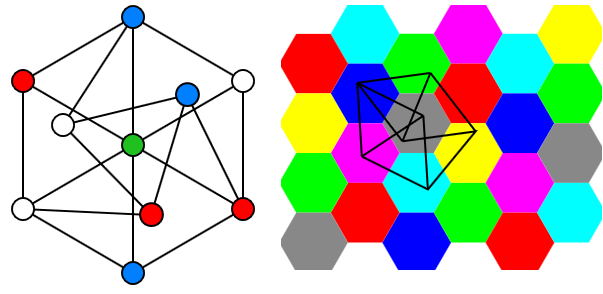
\includegraphics[scale=0.4]{images/Chromatic_plane.png}
\end{center}
\newpage{}

\section{(8) Хроматическое число пространства. Нижняя оценка $(c + o(1))^{dim}$}
\Def Хроматическое число пространства - min количество цветов, в которое можно так покрасить все точки этого пространства, чтобы между точками одного цвета не было расстояния 1:

$\chi(\R^n) = min \{\chi: \R^n = V_1 \sqcup V_2 \sqcup \dots \sqcup V_{\chi} : \forall i, \forall \overline{x}, \overline{y} \in V_i |\overline{x} - \overline{y}| \neq 1 \}$

\Example $\chi(\R) = 2$, просто красим полуинтервалы длины 1 в разные цвета.

\Th $\chi(\R^n) \geqslant (c + o(1))^{dim}$

\Proof
$G(n, 3, 1)$ - граф из 9 билета. Очевидно, что $\chi(\R^n) \geqslant \chi(G(n, 3, 1)) \geqslant \frac{|V|}{\alpha(G(n, 3, 1))} = \frac{C_n^3}{m(n, 3, 1)} \geqslant \frac{C_n^3}{n} \sim \frac{n^2}{6} $. 

Теперь перейдём к более общему случаю $G(n, r, s)$:

$\chi(\R^n) \geqslant \chi(G(n, r, s)) \geqslant \frac{C_n^r}{m(n, r, s)}$

Заметим, что расстояние между двумя рёбрами $G(n, r, s)$ равно $\sqrt{2(r-s)}$ (просто расписать расстояние между векторами).

Теперь максимизируем правую дробь. Возьмём $r = r(n) \sim \frac{2 - \sqrt{2}}{2} \cdot n$ (можно сделать r целой частью от этой же штуки), $s\sim \frac{r}{2}$
Это расстояние должно быть простым числом $p$. Из курса ОКТЧ мы всегда можем выбрать простое число в отрезке $[x, x+O(x^{0.525})]$ при достаточно больших значениях, т.е. мы найдём подходящее нам простое число.

$\frac{C_n^{[\frac{2 - \sqrt{2}}{2}]}}{\sum_{k=0}^{p-1} C_n^k}$

$a = \frac{2 - \sqrt{2}}{2}$, тогда 

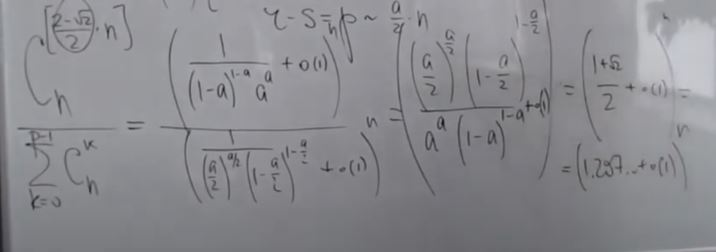
\includegraphics[]{images/71_2.JPG}
\EndProof
\newpage{}

\section{(8) Проблема Борсука. Подсчёт числа Борсука для прямой и плоскости.}
Проблема Борсука: $\Omega \subset \R^n, diam \Omega = sup_{x, y \in \Omega} |x - y| < \infty$.

Borsuk, 1933: $\Omega = \Omega_1 \sqcup \Omega_2 \sqcup \dots \sqcup \Omega_f$, $diam \Omega_i < diam \Omega$, $f(\Omega) = $ min число частей, на которое можно разбить $\Omega$; $f(n) = max_{\Omega} f(\Omega)$.

б.о.о. можно считать, что $diam \Omega = 1$, т.к. остальные мы тогда тоже научимся получать; $\Omega$ можно считать замкнутым, так как от точек на границе не поменяется диаметр. Более того, можно даже считать выпуклым (брать выпуклую оболочку), строгое док-во не нужно.

На прямой ($\R$): очевидно, берём $\Omega$, накрываем отрезком длины 1, разделяем пополам, очевидно, что диаметр стал меньше. Таким образом, $f(1) = 2$.

На плоскости ($\R^2$): очевидно, что $f(2) \geqslant 3$: берём 3 точки, которые вершины равностороннего треугольника (аналогично доказывается, что $f(n) \geqslant n + 1$).

Докажем, что $f(2) \leqslant 3$. 

\Statement Любое выпуклое множество диаметра 1 можно загнать в шестиугольник с расстоянием между противоположными сторонами 1. (термин: покрышка)

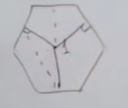
\includegraphics[]{images/72.JPG} 

И вот этими расстояниями она разбивается на три части, диаметры которых меньше 1.

\Proof

Возьмём произвольную прямую, не имеющую общих точек с $\Omega$. Строим параллельную ей прямую, которая бы касалась с $\Omega$ и ещё одну, как бы с 2х сторон. С этим всё хорошо, т.к. мн-во выпуклое. Далее достраиваем это до шестиугольника с углами по 120 градусов, а расстояние между параллельными сторонами не более 1.

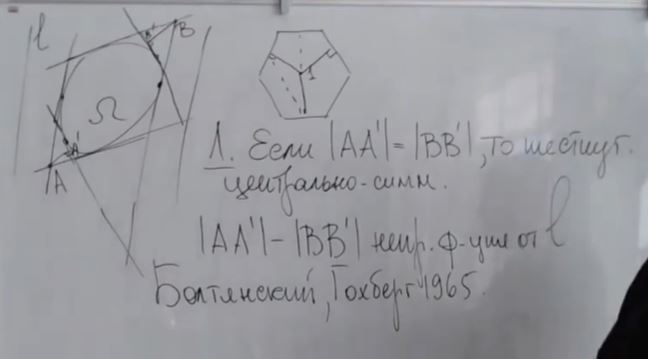
\includegraphics[]{images/72_3.JPG}

Таким образом, раз функция этих расстояний непрерывна и в начале больше 0, а в конце меньше 0, то будет такое положение прямой $l$, когда значение функции равно 0, значит, мы получим правильный шестиугольник.

\EndProof
\newpage{}

\section{(10) Проблема Борсука. Нижняя оценка числа Борсука \texorpdfstring{$(c + o(1))^{\sqrt{dim}}$}{(c+o(1))^sqrt(dim)}.}
Проблема Борсука: $\Omega \subset \R^n, diam \Omega = sup_{x, y \in \Omega} |x - y| < \infty$.

Borsuk, 1933: $\Omega = \Omega_1 \sqcup \Omega_2 \sqcup \dots \sqcup \Omega_f$, $diam \Omega_i < diam \Omega$, $f(\Omega) = $ min число частей, на которое можно разбить $\Omega$; $f(n) = max_{\Omega} f(\Omega)$.

б.о.о. можно считать, что $diam \Omega = 1$, $\Omega$ можно считать замкнутым, выпуклым.

\Th $f(n) \geqslant (c + o(1))^{\sqrt{n}}, c \approx 1.203$

\Proof
p - простое; $n = 4p$; $V = \{\overline{x} = (x_1, \dots, x_n) : x_i \in \{+1, -1\}, x_1 = 1, x_2 \cdot \dots \cdot x_n = 1\}$

$|V| = 2^{n-2}$

\Lemma 1: $\forall x, y \in V: (x, y) \equiv 0 (4)$

\Lemma 2: $\forall x, y \in V: (x, y) \equiv 0 (p)$, p нечёт. Но тогда верно $\forall x, y \in V (x, y) = 0 || x = y$.

\Lemma 3: Пусть $W \subset V$: $\forall x, y \in W (x, y) \neq 0$. Тогда $|W| \leqslant \sum_{k=0}^{p-1}C_n^k$

Докажем лемму 3. Пусть $W = \{x_1, \dots, x_t\}$, $(x_i, x_j) \neq 0 \Leftrightarrow (x_i, x_j) \notequiv 0 (p)$. Тогда $x_i \to P_{x_i} \in \Z_p[y_1, \dots, y_n]: P_{x_i}(y) = \prod_{j=1}^{p=1} (j - (x_i, y))$. Модифицируем моном (редуцируем степени): удаляем все чётные степени, а вместо нечётных оставляем 1. Ура.

Используя лемму, построим контрпримеры и получим нижнюю оценку. Модифицируем $V$: $V \to V^* \subset \R^{n^2}$: $x = (x_1, \dots, x_n) \in V \to x^* = (x_1^2, x_1x_2, \dots, x_n^2) \in V^*$; соответствие взаимно однозначное, т.к. $x_1 = 1$, так как отрезок из первых $n$ элементов равен исходному вектору.

В силу того, что некоторые координаты у $x^*$ всегда равны 1 или то, что $x_ix_j = x_jx_i$ мы можем снизить размерность до $\R^{C_n^2}$

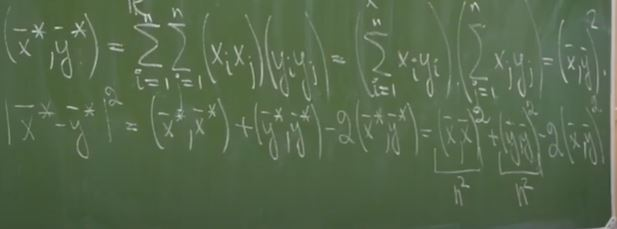
\includegraphics[]{images/73.JPG}

Таким образом, чтобы получить диаметр в $V^*$ нам нужно, чтобы $(x, y) = 0$.

$V = V_1^* \sqcup V_2^* \sqcup \dots \sqcup V_f^*$. Предположим, что $f < \frac{2^{n-2}}{\sum_{k=0}^{p-1} C_n^k}$; $V = V_1 \sqcup V_2 \sqcup \dots \sqcup V_f$ $\Rightarrow$ $\exists i : |V_i| \geqslant \frac{|V|}{f}$ (принцип Дирихле) $ > \sum_{k=0}^{p-1} C_n^k$ $\Rightarrow \exists x, y \in V_i: (x, y) = 0$ (лемма 3) $ \Rightarrow $ соответствующие $x^*, y^*$ реализуют диаметр $V^*$. Тогда $f(V^*) \geqslant \frac{2^{n-2}}{\sum_{k=0}^{p-1} C_n^k}$ $\Rightarrow$ $f(C_n^2) \geqslant \frac{2^{n-2}}{\sum_{k=0}^{p-1} C_n^k}$; $C_n^2 = d, d \sim \frac{n^2}{2} \Rightarrow n \sim \sqrt{2d}$

$\sum_{k=0}^{p-1} C_n^k = (\frac{1}{(1/4)^{1/4}(3/4)^{3/4}} + o(1))^n$, тогда $\frac{2^{n-2}}{\sum_{k=0}^{p-1} C_n^k} = (1.139 + o(1))^n = (1.139^{\sqrt{2}} + o(1))^{\sqrt{d}} = (1.203 + o(1))^{\sqrt{d}}$
\EndProof
\newpage{}

\section{(10) Проблема изоморфизма графов. Полиномиальный алгоритм, работающий почти на всех графах: описание и доказательство корректности (лемма о вероятности события C¯ б/д).}
\Def Графы $G_1 = (V_1, E_1), G_2 = (V_2, E_2), G_1 \cong G_2$ ($G_1$ изоморфен $G_2$), если $\exists$ биекция $\varphi: V_1 \leftrightarrow V_2: \forall x, y: (x, y) \in E_1  (\varphi(x), \varphi(y)) \in E_2$

Проблема: всего различных изоморфных графов $n!$; нет решения проблемы в алгоритмическом ключе для всех графов на n вершинах (мы не можем получить полиномиальную асимптотику). 

Случайный граф $G(n, \frac{1}{2})$; хотим доказать, что есть алгоритм, который работает на почти всех графах за полиномиальное время. На почти всех значит, что доля графов, на которых не работает, стремится к нулю; таким образом, если $K_n$ - графы, на которых алгоритм работает верно, то $|K_n| = 2^{C_n^2(1 + o(1))}$

Авторы алгоритма: Эрдеш, Бабаи, Selkow. 

Каноническая нумерация.

1. Пусть $r = [3log_2n]$. Выберем в нём $r$ вершин наибольшей степени: $d(1) \geqslant d(2) \geqslant d(3) \geqslant \dots \geqslant d(r)$. Если где-то равенство, то граф не попадает в $K_n$ и алгоритм завершёл.

Рассмотрим $i = r+1, \dots , n$. Введём $f(i) = \sum_{j=1}^{r} a(i, j) \cdot 2^j$, где 

\begin{equation*}
a(i, j) = 
 \begin{cases}
   1 &\text{, если $(i, j) \in E$}\\
   0 &\text{, если $(i, j) \notin E$}
 \end{cases}
\end{equation*}

2. Далее упорядочиваем эти коды: $f(r + 1) \geqslant f(r+2) \geqslant \dots \geqslant f(n)$ и если вновь где-то стоит знак равенства, то наш граф не попадает в $K_n$ и алгоритм завершён; иначе добавляем в $K_n$ (и мы занумеровали каноническим способом).

Корректность: \Proof Пусть $C$ - событие: $\forall i: 1, \dots, r+2 d(i) \geqslant d(i+1) + 3 $ ; $C(i, j)$ - событие: при удалении вершин $i, j$ из G старшие по величине r степеней нового графа попарно различны. Получается, что $\forall i, j C \to C_(i, j)$ за счёт запаса.

\Lemma (б/д): $P(\overline{C}) \to 0, n \to \infty$. 

Событие $A(i, j)$: либо $C(i,j)$ не выполнено, либо $G$ отвергается алгоритмом из-за совпадения величин $f(i), f(j)$.

$P(G \notin K_n) \leqslant P(\overline{C}) + P(C \text{ и граф отвергается на 2 этапе})$; осталось убедиться, что $P(C \text{ и граф отвергается на 2 этапе}) \to \infty$, т.к. первое стремится к 0 по лемме. 

$P(C \text{ и граф отвергается на 2 этапе}) \leqslant \sum_{i < j} P(C(i, j) \cap A(i, j))\leqslant \sum_{i < j} P(A(i, j) | C(i, j)) \leqslant C_n^2 \cdot 
(\frac{1}{2})^r < n^2 2^{-3log_2n} = \frac{1}{n} \to 0$ \EndProof
\newpage{}